\documentclass[parskip]{iisreport}

\usepackage{pdfpages}
\usepackage{todonotes}
\usepackage[numbers]{natbib}

% Uncomment the following line to disable the todo notes.
% \usepackage[disable]{todonotes}

\lstset{numbers=left}

\title{Implementing an OpenMP runtime for MemPool in LLVM}

\author{Diego de los Santos Gausí}
\email{dgausi@student.ethz.ch}

\semester{Spring 2024}
\date{1st of July 2024}
\reporttype{Semester Project}

\professor{Prof.\ Dr.\ L.\ Benini, lbenini@iis.ee.ethz.ch}

\advisor{Samuel Riedel, sriedel@iis.ee.ethz.ch}
\advisor{Sergio Mazzola, smazzola@iis.ee.ethz.ch}

\titlelogo{titlepage_logo}
\titlelogoheight{7cm}

\begin{document}

% Format: \newacronym{handle}{acronym}{full term}
% The full term should be in title case for proper names and in sentence case otherwise.
% If in doubt about hyphenation or case style, refer to the English Wikipedia.
\newacronym{dma}{DMA}{Direct Memory Access}
\newacronym{axi}{AXI}{Advanced eXtensible Interface}
\newacronym{gcc}{GCC}{GNU Compiler Collection}
\newacronym{api}{API}{Application Programming Interface}
\newacronym{wfi}{WFI}{Wait For Interrupt}


\frontmatter

\listoftodos

\chapter*{Abstract}

In order to effectively harness MemPool's parallelism, an initial GCC-compatible OpenMP runtime was
developed for this architecture, supporting the most commonly used set of features. However, due to
increasing reliance on the LLVM compiler infrastructure by the MemPool team, it is becoming crucial
to have an OpenMP runtime compatible for it. This project aims to implement an OpenMP runtime that
works with LLVM, supporting at least the same set of features as the previous runtime, while
maintaining comparable performance and offering the possibility of future additions and
improvements.

% The abstract summarizes what this report is about.
% It focusses on the big picture and does not go into details.
% You should write concisely about the following points:
%
% \begin{itemize}
% 	\item Describe the \textbf{background} of your project: what is the motivation for your project and why is it important?
% 	\item Describe the \textbf{objectives} of your project.
% 	\item Describe the \textbf{problems} that must be addressed to achieve the objectives---why are these problems difficult?
% 	\item Describe your \textbf{approach} and \textbf{methods}.
% 	\item Summarize the most important \textbf{results}.
% 	\item State the main \textbf{conclusion} and its significance.
% \end{itemize}
%
% The abstract typically takes half a page and should not be longer than one full page.
% Try to write a draft of the abstract early on to have a good idea of your project, but revise the abstract as the project progresses.
% Write the final version of the abstract once the report is otherwise complete.
%
% The remainder of this document contains an example on structure and content of the report.
% This template is meant to guide you and not to force you into a certain structure---just make sure you and your advisors agree on content and structure of the report \emph{before} you start writing it.
% \Cref{app:topic-specific_guidelines} gives more specific guidelines for some major project areas (e.g., hardware designs).
% If you are new to \LaTeX{} or want to learn some best practices, you should also check the short \LaTeX{} guide in \cref{app:LaTeX_guide}.

\chapter*{Acknowledgments}

I'd like to sincerely thank Samuel Riedel and Sergio Mazzola for supervising this project. Their
continuous feedback and encouragement has been very helpful, and it enabled me to stay on track and
make steady progress.

I'd also like to thank Frank Gürkaynak for getting me in touch with the group, which led to me
learning about this project.

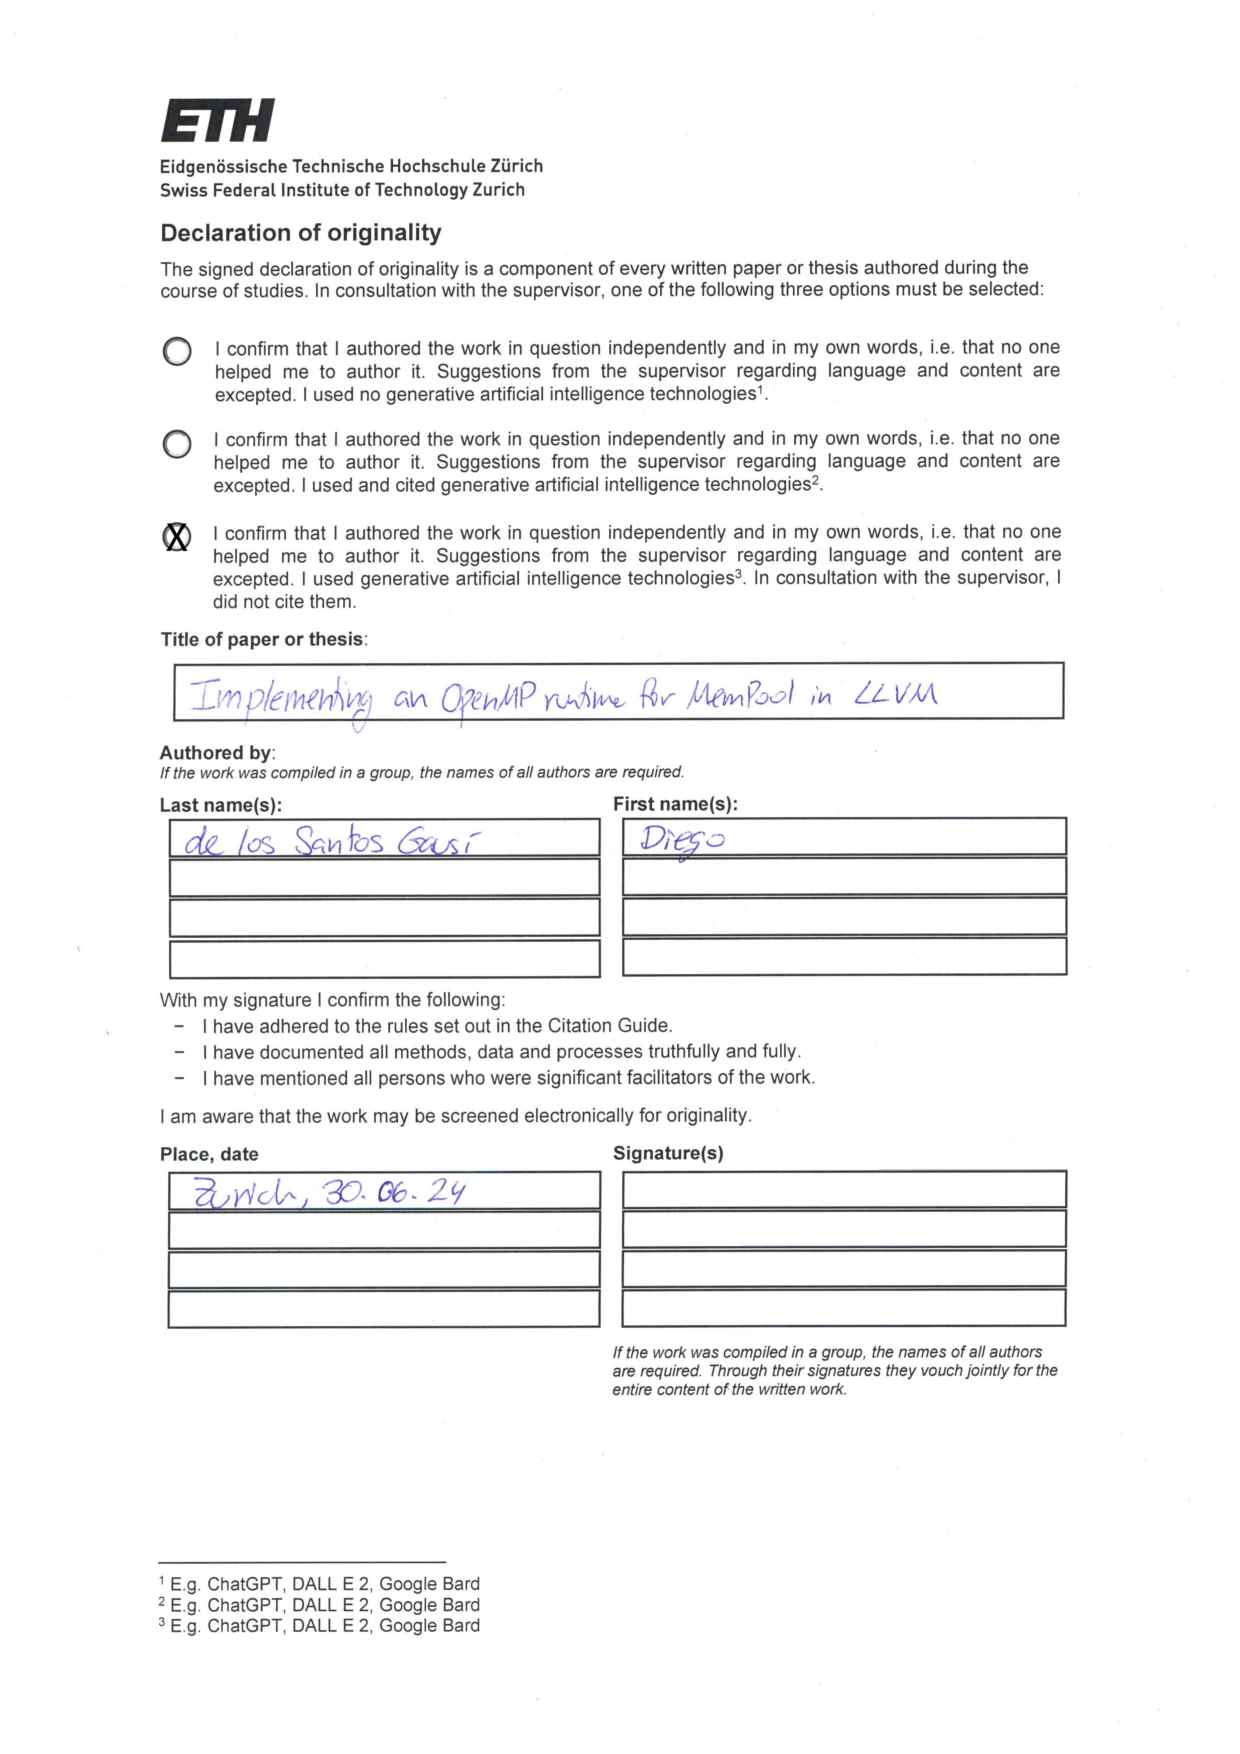
\includepdf[scale=0.9]{../declaration-originality-unsigned.pdf}

% {\color{red}
% Download the official declaration of originality\footnote{\url{https://www.ethz.ch/content/dam/ethz/main/education/rechtliches-abschluesse/leistungskontrollen/declaration-originality.pdf}}, print it, and sign it.
% When printing your thesis, replace this sheet with the physically signed original paper.
% For the digital version, scan the filled declaration of originality (either before signing or remove your signature\footnote{%
%   By removing your signature from the digital version of your report, you enable us to share your report with collaborators without having to deal with privacy concerns.
% } from the image) and replace the text inside this file with \verb|\includepdf[scale=0.9]{declaration_of_originality}|.
% }


\tableofcontents

\mainmatter

\chapter{Introduction} \label{ch:introduction}

MemPool~\cite{mempool} is an open-source manycore architecture developed at ETH. It is comprised of
up to 1024~\cite{terapool} 32-bit RISC-V Snitch~\cite{snitch} cores that share a common L1 cache.
Unlike on GPUs, each core is individually programmable, therefore enabling the familiar shared
memory programming model.

Although MemPool's parallelism can be harnessed by manually managing it using the primitives
provided by MemPool's C runtime library, this can become a tedious and error prone task since the
programmer has to be knowledgeable about the underlying architecture. Luckily, higher level
abstraction layers such as OpenMP~\cite{openmp} allow the programmer to express this parallelism in
a clear and concise way using the fork-join paradigm and without needing advanced architectural
knowledge.

OpenMP is comprised of a set of compiler directives for both C/C++ and Fortran that enable this
higher level abstraction. In order to use OpenMP, one has to use a compatible compiler that is able
to roughly do the following:

\begin{enumerate}
	\item The compiler must be able to parse the directives and compile the surrounding code
	      according to their semantics.
	\item The output of the compilation process must match the target platform in order to make use
	      of its parallelism capabilities and primitives.
\end{enumerate}

Both the \gls{gcc} and LLVM provide an OpenMP runtime library interface that bridges the gap between
both points: instead of directly generating a binary from OpenMP annotated code, the compiler
generates calls to the OpenMP runtime library. This library has to be aware of how to parallelize
the code given the platform, which makes it inherently non-portable. Naturally, popular compilers
ship with their own OpenMP runtime library implementation, however, in order to get around the
non-portability issue, they target a host running an operating system which is able to provide the
necessary parallelism primitives. Since MemPool is designed to run bare-metal applications, this
means that a custom OpenMP runtime library has to be developed.

Previously, the authors of MemPool developed a \gls{gcc} compatible OpenMP runtime library with
support for the most commonly used OpenMP constructs, such as \emph{work sharing}, \emph{critical
sections} and \emph{atomics}.\footnote{This implementation will be discussed in more detail in
\cref{sec:gcc_implementation}.} However, as the MemPool team increasingly relies on the LLVM
compiler infrastructure, it is essential to have a compatible OpenMP runtime library for LLVM as
well.

The goal of this project is to implement an OpenMP runtime for LLVM that works on MemPool, supports
at least the same set of features as the previous \gls{gcc} runtime and achieves comparable
performance.

The runtime will be implemented in C++ as detailed in \cref{ch:implementation}. In
\cref{ch:results}, the new runtime will be evaluated in terms of performance and correctness against
the \gls{gcc} runtime. Finally, we will summarize the results and discuss possible shortcomings and
future work in \cref{ch:conclusion}.

% The introduction motivates your work and puts it into a bigger context. It should answer the
% following questions: What is the background of this work? What is the state of the art? Why is
% this project necessary to advance the state of the art? What are the problems that have to be
% solved and why are they difficult? What are your contributions to solve these problems? How do you
% evaluate your solution to show that it is adequate and applicable?
%
% An introduction written along these questions naturally follows the \textit{\gls{spse}}\footnote{%
% The \acrshort{spse} approach was established in a book~\cite{Hoey83}, but is also briefly
% summarized in a more recent article~\cite{MP12}, which is available online. } approach. In the
% \emph{situation}, you set the scene for your work and catch the interest of the readers by showing
% the importance and generality of the scene. In the \emph{problem}, you spot an issue in the scene
% and show why and how it significantly taints the scene. In the \emph{solution}, you outline your
% solution to that issue. Finally, in the \emph{evaluation}, you present the main arguments why the
% claimed solution actually does solve the problem.
%
% In the following chapters, you will elaborate each of the four \gls{spse} elements in detail: In
% \textsl{Background}, you lay the foundations for an in-depth understanding of the situation and
% the problem. In \textsl{Related Work}, you show how others have address this (or similar) problems
% and why their solutions are not sufficient or applicable. In \textsl{Implementation}, you specify
% your solution, which you then evaluate rigorously for strengths and weaknesses in
% \textsl{Results}.
%
% At the end of the introduction, you should explicitly show this structure to the reader by briefly
% explaining how this report is organized. Instead of using the general \gls{spse} terminology and
% the chapter names mentioned above, we urge you to use the domain-specific terminology established
% in the introduction and point to chapters using cross references (e.g., refering to
% \cref{ch:background} instead of ``the Background chapter'').

\chapter{Background}
\label{ch:background}

{\color{red}
	Explain the background and theory underlying your project.
	Assume that the average reader has the same knowledge you had \emph{before} undergoing this project.
	This chapter should transfer all knowledge necessary to understand the following chapters.

	As this and the following chapters are likely longer than a few pages, consider structuring them into sections (but avoid fragmentation by overly fine-grained sectioning).
	Use the \verb|\..section{}| command family as illustrated below:

	\section{First section}
	\label{sec:background_overview}

	\subsection{First subsection}

	\subsection{Second subsection}

	\subsubsection{First subsubsection}

	Follow a top-down approach when structuring the chapter, and guide the reader by giving a short overview at the beginning of each section.
	Again, you can use labels and references (e.g., referring to \cref{sec:background_overview}).
}

\chapter{Related Work}
\label{ch:related_work}

\begin{itemize}
  \item HERO LLVM implementation
  \item Previous gcc (?)
\end{itemize}

{\color{red}
	Discuss the state-of-the art and other related work.
	Depending on how much related work exists and how central the comparison to it is in your thesis (discuss this with your advisors), the introduction may contain sufficient related work and this chapter can be omitted.
}

\chapter{Implementation}
\label{ch:implementation}

\begin{itemize}
  \item Top down explanation of the implementation, including different iterations and why they
        were discarded
  \item Minor things like the testing scripts and main function wrapper
\end{itemize}

{\color{red}
	This chapter explains your contributions, be it algorithms, architectures, libraries, hardware, or others.
	As usual, follow a top-down approach and break the chapter into meaningful sections.
	It may even be necessary to split the chapter into multiple chapters (e.g., to separate architecture from implementation in a hardware design).

	Derive a structure for this chapter that is meaningful for your report and discuss it with your advisors.
}

\chapter{Results}
\label{ch:results}

\section{Evaluation setup}

For our evaluation, we simulate a MemPool \gls{soc} in its \emph{MinPool} (16-core) configuration
using the Verilator~\cite{verilator} simulator. Additionally, we increase the stack size for each
core to 1024 bytes to accommodate the higher stack usage of the new runtime, and disable the
\texttt{Xpulp} instructions, since they are not fully supported when compiling with LLVM.

In order to compare the performance of the new runtime against the previous one, we run a part of
the existing benchmarks available in the MemPool
repository\footnote{\url{https://github.com/pulp-platform/mempool}} using both of them.

For correctness, we run the set of tests also provided in the MemPool repository, however, we adapt
them to use the new testing framework described in the following section. Additionally, we add new
tests for the \texttt{teams} and \texttt{sections} constructs, which we describe in more detail in
\cref{sec:correctness}.

\subsection{Testing Framework}
\label{subsec:testing-framework}

The testing framework consists of a small set of C preprocessor macros that allow us to make
assertions, define test cases and run them. It is inspired by \citeauthor{minunit}'s minimal testing
framework~\cite{minunit}.

It is comprised of the following macros:

\begin{itemize}
	\item \texttt{ASSERT_TRUE(condition, error_message)}: Checks that \texttt{condition} evaluates to
	      \texttt{true}. If it does not, it prints \texttt{error_message} and fails the test.
	\item \texttt{ASSERT_EQ(left, right)}: Checks that \texttt{left} is equal to \texttt{right}. If
	      it is not, it prints an error message and fails the test.
	\item \texttt{ASSERT_NEQ(left, right)}: Checks that \texttt{left} is not equal to \texttt{right}.
	      If it is, it prints an error message and fails the test.
	\item \texttt{EXPECT_TRUE(condition, error_message)}: Similar to \texttt{ASSERT_TRUE}, but does
	      not fail the test if the condition is not met, it only prints the error message.
	\item \texttt{TEST(testname)}: Defines a new test with the name \texttt{testname} and adds it to
	      the list of tests to be run.
	\item \texttt{RUN_TEST(testname)}: Runs the test \texttt{testname}.
	\item \texttt{RUN_ALL_TESTS()}: Runs all tests defined in the test suite.
	\item \texttt{PRINT_TEST_RESULTS()}: Prints the results of the test suite (i.e., how many tests
	      were run and how many failed).
\end{itemize}

When printing, the framework includes easy to parse markers to the output such as, \texttt{[FAIL]}
or \texttt{[SUCCESS]}, which can be used by, e.g., a python script to run multiple tests in
succession and automatically show the results to the user.

\section{Correctness}
\label{sec:correctness}

Our implementation passes all of the correctness tests provided in the MemPool repository, as well as
the new tests described in the following sections.

\subsection{\texttt{teams} Construct}

The test shown in \cref{lst:test-teams-distribute} checks that the \texttt{teams distribute}
construct correctly distributes the iterations of the loop across the teams. It does so by checking
that the team number is correct for each iteration. It also checks that the number of teams matches
the number of requested teams by comparing the value returned by \texttt{omp\_get\_num\_teams()} to
the expected value (4).

\begin{lstlisting}[language=C, caption={test_teams_distribute}, label={lst:test-teams-distribute}]
TEST(test_teams_distribute) {
  for (int rep = 0; rep < REPETITIONS; rep++) {
    int num_teams = 0;
    int team_num[12];

#pragma omp teams distribute num_teams(4)
    for (int i = 0; i < 12; i++) {
      team_num[i] = omp_get_team_num();

      if (omp_get_team_num() == 0) {
        num_teams = omp_get_num_teams();
      }
    }

    for (int i = 0; i < 12; i++) {
      ASSERT_EQ(team_num[i], i / 3);
    }

    ASSERT_EQ(num_teams, 4);
  }
}
\end{lstlisting}

The test shown in \cref{lst:test-teams-reduce} checks that each team is able to work independently
by performing a reduction onto a team-local variable. The result of each reduction is then compared
against the expected value (32).

\begin{lstlisting}[language=C, caption={tests_teams_reduce}, label={lst:test-teams-reduce}]
TEST(test_teams_reduce) {
  for (int rep = 0; rep < REPETITIONS; rep++) {
    int sum[4];

#pragma omp teams num_teams(4)
    {
      int local_sum = 0;

#pragma omp parallel for reduction(+ : local_sum)
      for (int i = 0; i < 32; i++) {
        local_sum += 1;
      }

      sum[omp_get_team_num()] = local_sum;
    }

    for (int i = 0; i < 4; i++) {
      ASSERT_EQ(sum[i], 32);
    }
  }
}
\end{lstlisting}

Finally, the test shown in \cref{lst:test-teams-barrier} checks that barriers work correctly within
teams and don't affect other teams. It does so by performing an independent barrier test in each
team, that checks that the barrier is functional.

\begin{lstlisting}[language=C, caption={test_teams_barrier}, label={lst:test-teams-barrier}]
TEST(test_teams_barrier) {
  for (int rep = 0; rep < REPETITIONS; rep++) {
    int results[2];
#pragma omp teams num_teams(2)
    {
      uint32_t team_num = omp_get_team_num();
      int result = 0;

#pragma omp parallel
      {
        uint32_t rank = omp_get_thread_num();
        if (rank == 1) {
          mempool_wait(1000);
          result = 3;
        }
#pragma omp barrier

        if (rank == 2) {
          results[team_num] = result;
        }
      }
    }

    ASSERT_EQ(results[0], 3);
    ASSERT_EQ(results[1], 3);
  }
}
\end{lstlisting}

\subsection{\texttt{sections} Construct}

The test shown in \cref{lst:test-sections} checks that the \texttt{sections} construct correctly
distributes the sections across the threads. It does so by checking that each section is executed by
a different thread.

\begin{lstlisting}[language=C, caption={test_omp_parallel_sections}, label={lst:test-sections}]
TEST(test_omp_parallel_sections) {
  for (int rep = 0; rep < REPETITIONS; rep++) {
    uint32_t section_1 = 0;
    uint32_t section_2 = 0;

#pragma omp parallel sections
    {

#pragma omp section
      { section_1 = omp_get_thread_num(); }

#pragma omp section
      { section_2 = omp_get_thread_num(); }
    }

    ASSERT_NEQ(section_1, section_2);
  }
}
\end{lstlisting}

\section{Performance}

To account for performance differences that arise purely from using different compilers, we compare
the performance of the new runtime against the previous one in two different ways:

First, we obtain the speedup of running a given workload in parallel versus sequentially with the
same compiler, and compare this across runtimes. This way, the effect of a more performant
compilation output will be mitigated, since the speedup is calculated relative to the sequential
baseline. The results of this approach will be discussed in \cref{subsec:speedup}.

Then, we look at the cost of specific runtime operations (e.g., barriers, startup time, etc.)
and compare them across runtimes as well. This way we can isolate individual components and see
if any of them could benefit from further optimizations. The results of this approach will be
discussed in \cref{subsec:runtime-overhead}.

\subsection{Speedup}
\label{subsec:speedup}

\subsubsection{Sparse Matrix-Vector Multiplication}

In this benchmark, we perform \gls{spvm}, where the matrix is stored in
\gls{csr} format. It has 512 columns and we vary the number of rows from 1 to 512.

\begin{figure}[h]
	\centering
	\begin{minipage}{0.49\textwidth}
		\centering
		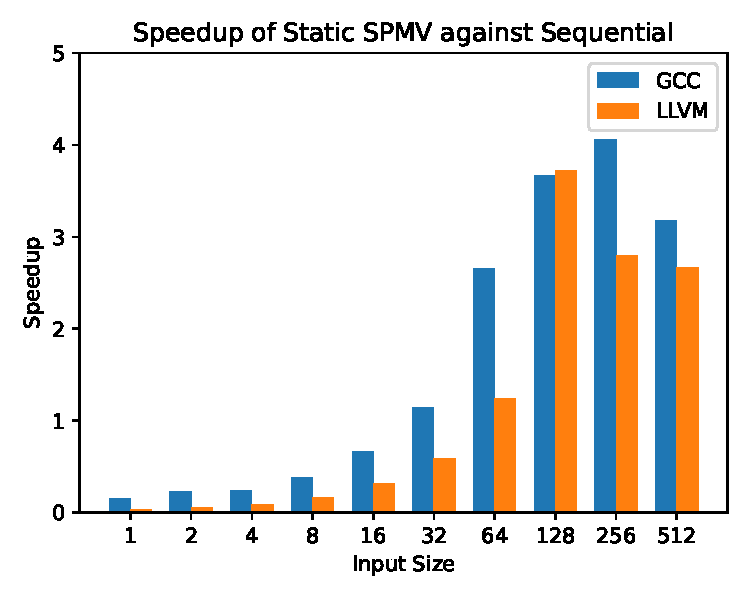
\includegraphics[width=\linewidth]{./fig/benchmarks/spvm_speedup_static.pdf}
		\caption{Static SPVM Speedup.}%
		\label{fig:spvm-static-speedup}
	\end{minipage}\hfill
	\begin{minipage}{0.49\textwidth}
		\centering
		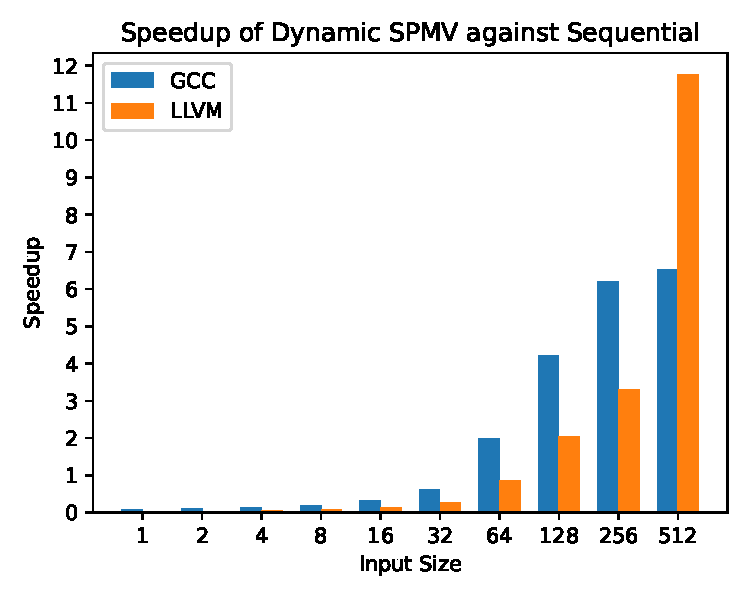
\includegraphics[width=\linewidth]{./fig/benchmarks/spvm_speedup_dynamic.pdf}
		\caption{Dynamic SPVM Speedup.}%
		\label{fig:spvm-dynamic-speedup}
	\end{minipage}
\end{figure}

\subsubsection{Matrix-Matrix Multiplication}

In this benchmark, we perform \gls{mmm} of square matrices, where we vary the
size of both matrices from 1 to 32.

\begin{figure}[h]
	\centering
	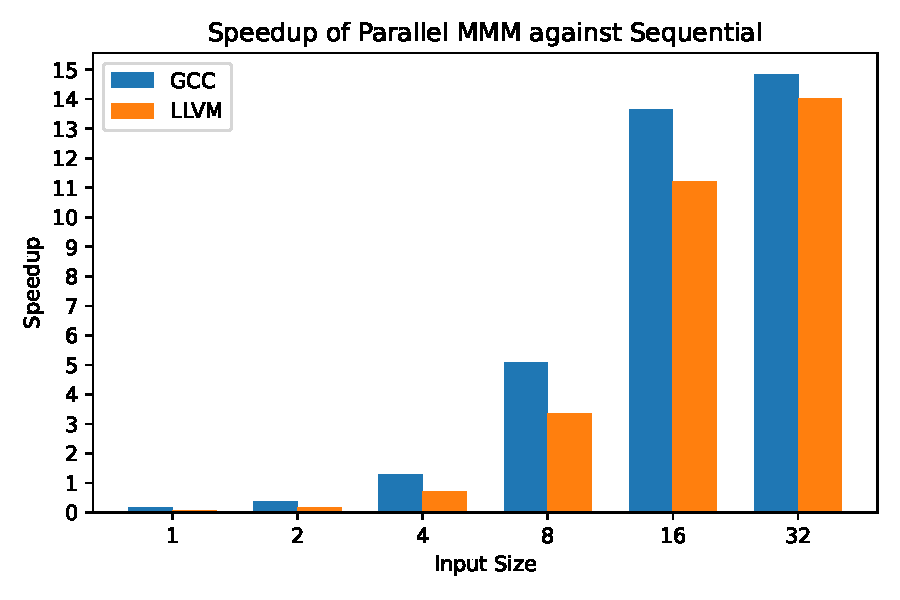
\includegraphics[width=.59\linewidth]{./fig/benchmarks/mm_speedup.pdf}
	\caption{Matrix-Matrix Multiplication Speedup.}%
	\label{fig:mm-speedup}
\end{figure}

\subsubsection{Dot Product}

In this benchmark, we perform the dot product of two vectors of size 1 to 2048.

\begin{figure}[h]
	\centering
	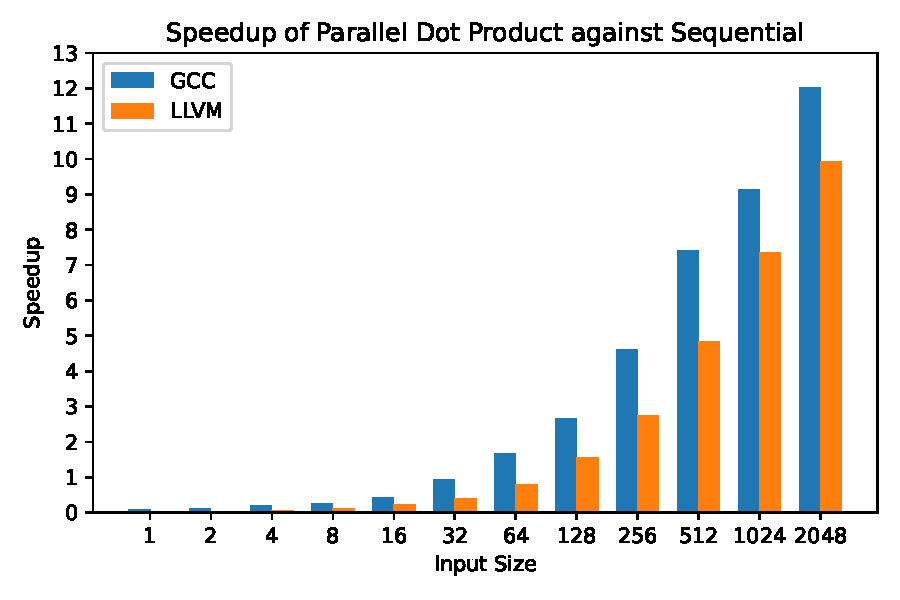
\includegraphics[width=.59\linewidth]{./fig/benchmarks/dotp_speedup.pdf}
	\caption{Dot Product Speedup.}%
	\label{fig:dotp-speedup}
\end{figure}

\subsection{Runtime Overhead}
\label{subsec:runtime-overhead}

\subsubsection{Startup Time}

We measure the runtime startup time using the benchmark shown in \cref{lst:benchmark-startup-time}. A
timer is started before executing the parallel region and stopped by the master thread inside a
master construct. We do this because the master thread is the one that performs the fork and we can
therefore know that when the master thread stops the timer, all of the other threads have at least
been initialized. The duration is averaged across 100 repetitions.

\begin{lstlisting}[language=C, caption={Startup Time Benchmark},
                   label={lst:benchmark-startup-time}]
void startup_time() {

  uint32_t duration = 0;

  for (int i = 0; i < REPETITIONS; i++) {

    mempool_timer_t cycles = mempool_get_timer();
    mempool_start_benchmark();

    #pragma omp parallel
    {

      #pragma omp master
      {
        mempool_stop_benchmark();
        cycles = mempool_get_timer() - cycles;
        duration += cycles;
      }
    }
  }

  printf("Startup time duration: %d\n", duration / REPETITIONS);
}
\end{lstlisting}

The results of the benchmarks are shown in \cref{tbl:benchmark-startup-time}, where we can see that
the new runtime has a startup time that is more than twice as long as the previous one.

\begin{table}[h]
	\centerfloat
	\begin{tabular}{ r r r r }
		\toprule
		\textbf{Runtime} & \textbf{Startup Time (cycles)} & \textbf{Speedup (vs. GCC)} \\
		\midrule
		GCC              & 154                            & 1                          \\
		LLVM             & 355                            & 0.43                       \\
		\bottomrule
	\end{tabular}
	\caption{Startup Time Benchmark Results.}%
	\label{tbl:benchmark-startup-time}
\end{table}

\subsubsection{Barrier}

In this benchmark, we measure the number of cycles it takes to execute an increasing number of
barriers, as shown in \cref{lst:benchmark-barrier}.

\begin{lstlisting}[language=C, caption={Barrier Benchmark},
                   label={lst:benchmark-barrier}]
int main() {
#pragma omp parallel
  {
    unsigned int counter = 0;
    unsigned int cycles = 0;
    unsigned int start_time = 0;

    for (int i = 1; i < MAX_BARRIERS + 1; i++) {

#pragma omp barrier

      start_time = mempool_get_timer();
      mempool_start_benchmark();

      for (int j = 0; j < i; j++) {
#pragma omp barrier
        counter++;
      }

      mempool_stop_benchmark();
      cycles = mempool_get_timer() - start_time;

#pragma omp single
      printf("%d barriers: %d cycles\n", i, cycles);
    }
  }

  return 0;
}
\end{lstlisting}

As expected, the number of cycles increases linearly with the number of barriers, as shown in
\cref{fig:barrier-benchmark-cycles}. The execution time of a barrier using the new runtime is about
18\% faster than with old one, as shown in \cref{fig:barrier-benchmark-speedup}. \todo{Explain why
	for one barrier it is faster}

\begin{figure}[h]
	\centering
	\begin{minipage}{0.49\textwidth}
		\centering
		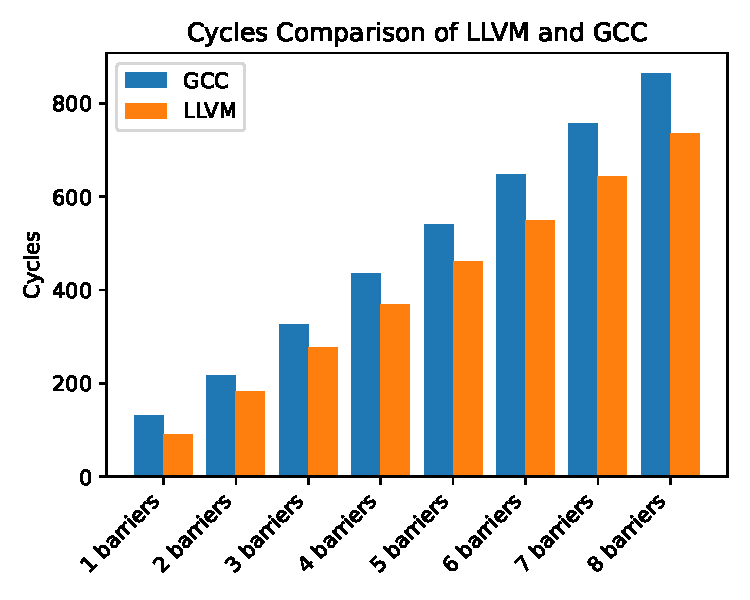
\includegraphics[width=\linewidth]{./fig/benchmarks/barrier_benchmark_cycles.pdf}
		\caption{Barrier Benchmark Cycles.}%
		\label{fig:barrier-benchmark-cycles}
	\end{minipage}\hfill
	\begin{minipage}{0.49\textwidth}
		\centering
		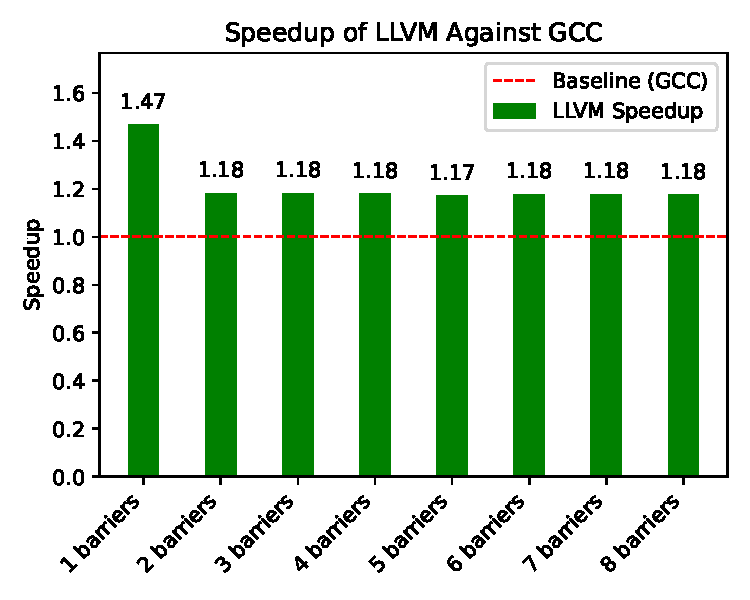
\includegraphics[width=\linewidth]{./fig/benchmarks/barrier_benchmark_speedup.pdf}
		\caption{Barrier Benchmark Speedup.}%
		\label{fig:barrier-benchmark-speedup}
	\end{minipage}
\end{figure}

\subsubsection{Critical Section}

In this benchmark, we measure the number of cycles it takes to execute a \texttt{critical} section,
as shown in \cref{lst:benchmark-critical}. The timer is started before the critical section and
stopped right after it is done executing. The master thread then aggregates the duration of each run
to finally print the average over 100 repetitions.

\begin{lstlisting}[language=C, caption={Critical Benchmark},
                   label={lst:benchmark-critical}]
void omp_parallel_critical() {
  uint32_t num_cores = mempool_get_core_count();
  uint32_t duration = 0;

  for (int i = 0; i < 100; i++) {

#pragma omp parallel num_threads(num_cores)
    {
      mempool_timer_t cycles = mempool_get_timer();
      mempool_start_benchmark();

#pragma omp critical
      { result += 100; }

      mempool_stop_benchmark();
      cycles = mempool_get_timer() - cycles;

#pragma omp master
      { duration += cycles; }
    }
  }

  printf("OMP Critical Duration: %d\n", duration / 100);
}
\end{lstlisting}

As shown in \cref{tbl:critical}, the new runtime achieves comparable performance in this benchmark,
needing less than 10 extra cycles to execute a critical section.

\begin{table}[h]
	\centerfloat
	\begin{tabular}{ r r r r }
		\toprule
		\textbf{Runtime} & \textbf{Critical Section (cycles)} & \textbf{Speedup (vs. GCC)} \\
		\midrule
		GCC              & 74                                 & 1                          \\
		LLVM             & 82                                 & 0.9                        \\
		\bottomrule
	\end{tabular}
	\caption{Critical Section Benchmark Results.}%
	\label{tbl:critical}
\end{table}

\subsubsection{Single Construct}

This benchmark follows the same structure as the previous one, except that the \texttt{critical}
section is replaced by a \texttt{single} construct.

\begin{lstlisting}[language=C, caption={Single Benchmark},
                   label={lst:benchmark-single}]
void omp_parallel_single() {
  uint32_t num_cores = mempool_get_core_count();
  uint32_t duration = 0;

  for (int i = 0; i < 100; i++) {

#pragma omp parallel num_threads(num_cores)
    {
      mempool_timer_t cycles = mempool_get_timer();
      mempool_start_benchmark();

#pragma omp single
      { result += 100; }

      mempool_stop_benchmark();
      cycles = mempool_get_timer() - cycles;

#pragma omp master
      { duration += cycles; }
    }
  }

  printf("OMP Single Duration: %d\n", duration / 100);
}
\end{lstlisting}

As shown in \cref{tbl:single}, the new runtime achieves a speedup of around 5.73 in this benchmark
compared to the previous one. This is because the \texttt{single} construct is implemented in a
completely different way: The GOMP runtime uses a global \texttt{work_t} struct (\cref{lst:work-t})
to signal to every thread whether the \texttt{single} construct has already been executed. This
requires locking, since all threads are trying to access it concurrently. Contrary to that, the new
runtime implements \texttt{single} constructs the same way as \texttt{master} constructs, which just
requires checking the thread's ID.

\begin{table}[h]
	\centerfloat
	\begin{tabular}{ r r r r }
		\toprule
		\textbf{Runtime} & \textbf{Single Construct (cycles)} & \textbf{Speedup (vs. GCC)} \\
		\midrule
		GCC              & 837                                & 1                          \\
		LLVM             & 146                                & 5.73                       \\
		\bottomrule
	\end{tabular}
	\caption{Single Construct Benchmark Results.}%
	\label{tbl:single}
\end{table}

\subsubsection{Master Construct}

This benchmark follows the same structure as the previous one, except that the \texttt{single}
construct is replaced by a \texttt{master} construct.

\begin{lstlisting}[language=C, caption={Master Benchmark},
                   label={lst:benchmark-master}]
void omp_parallel_master() {
  uint32_t num_cores = mempool_get_core_count();
  uint32_t duration = 0;

  for (int i = 0; i < 100; i++) {

#pragma omp parallel num_threads(num_cores)
    {
      mempool_timer_t cycles = mempool_get_timer();
      mempool_start_benchmark();

#pragma omp master
      { result += 100; }

      mempool_stop_benchmark();
      cycles = mempool_get_timer() - cycles;

#pragma omp master
      { duration += cycles; }
    }
  }

  printf("OMP Master Duration: %d\n", duration / 100);
}
\end{lstlisting}

A shown in \cref{tbl:master}, the new runtime achieves only about half of the performance of the
previous runtime.

\begin{table}[h]
	\centerfloat
	\begin{tabular}{ r r r r }
		\toprule
		\textbf{Runtime} & \textbf{Master Construct (cycles)} & \textbf{Speedup (vs. GCC)} \\
		\midrule
		GCC              & 38                                 & 1                          \\
		LLVM             & 69                                 & 0.55                       \\
		\bottomrule
	\end{tabular}
	\caption{Master Construct Benchmark Results.}%
	\label{tbl:master}
\end{table}

\todo{Try to explain difference between single and master for LLVM since they are implemented the
	same way}

\chapter{Conclusion and Future Work}
\label{ch:conclusion}

{\color{red}
	Draw your conclusions from the results and summarize your contributions.
	Point out aspects that need to be investigated further.

	The conclusion can be structured inversely to the introduction:
	Summarize how the \emph{evaluation} backs the \emph{solution}, which solves the \emph{problem}.
	Describe how your contributions improve the \emph{situation} and what other (potentially newly discovered) problems have to be solved in the future.

	Be concise: the conclusion normally fits on a single page and is rarely longer than two pages.
}


\appendix

\chapter{Implementation Details}

\section{KMP Entrypoints}
\label{sec:kmp-entrypoints}

\subsection{Parallel Construct}
\label{subsec:parallel-construct}

\subsubsection{\texttt{\_\_kmpc\_fork\_call}}
\label{subsubsec:kmpc-fork-call}

\paragraph{Description} This function is called by the master thread of the current team (the
default team contains all cores and the core with ID 0 runs the master thread). It is responsible
for assigning the appropriate number of threads to the team and waking them up, as well as setting
up the task that they will run.

\paragraph{Arguments}
\begin{itemize}
	\item \texttt{loc}: Pointer to a struct containing information about the source code location
	      of the call.
	\item \texttt{argc}: Number of arguments passed to the microtask function.
	\item \texttt{microtask}: Function pointer to the task to be run by each thread in the team.
	\item \texttt{...}: Variable number of arguments to be passed to the microtask function.
\end{itemize}

\paragraph{Implementation} First, it creates a \texttt{kmp::Task} (\cref{subsec:task}) object with
the microtask, arguments casted to a void pointer array, and the number of such arguments. Then, it
obtains the object representing the current thread using \texttt{kmp::runtime::getCurrentThread()}
(\cref{subsec:runtime-namespace}) and calls the \texttt{forkCall} method on it with the task as an
argument.

\begin{lstlisting}[language=C, caption={\_\_kmpc\_fork\_call}, label={lst:fork-call},
                   escapechar=@]
void __kmpc_fork_call(ident_t *loc, kmp_int32 argc,
                      kmpc_micro microtask, ...) {
  va_list args;
  va_start(args, microtask);
  kmp::Task kmpMicrotask(microtask, reinterpret_cast<void **>(args),
                         argc);
  kmp::runtime::getCurrentThread().forkCall(kmpMicrotask);
  va_end(args);
};
\end{lstlisting}

\subsubsection{\texttt{\_\_kmpc\_push\_num\_threads}}
\label{subsubsec:kmpc-push-num-threads}

\paragraph{Description} This function is called when using the \texttt{num\_threads} clause in a
parallel construct. It is used to request a specific number of threads to be used in the parallel
section.

\paragraph{Arguments}
\begin{itemize}
	\item \texttt{loc}: Pointer to a struct containing information about the source code location
	      of the call.
	\item \texttt{global\_tid}: Global ID of the calling thread.
	\item \texttt{num\_threads}: Requested number of threads.
\end{itemize}

\paragraph{Implementation} This function essentially just calls the \texttt{requestNumThreads}
method on the object representing the current thread (\cref{subsec:thread}), which sets the
\texttt{requestedNumThreads} field, obtained by calling \texttt{kmp::runtime::getThread}
(\cref{subsec:runtime-namespace}) with \texttt{global\_tid}.

\begin{lstlisting}[language=C, caption={\_\_kmpc\_push\_num\_threads}, label={lst:push-num-threads},
                   escapechar=@]
void __kmpc_push_num_threads(ident_t *loc, kmp_int32 global_tid,
                             kmp_int32 num_threads) {
  kmp::runtime::getThread(global_tid).requestNumThreads(num_threads);
};
\end{lstlisting}

\subsection{Work Sharing Constructs}

The following entrypoints are used when running work sharing constructs such as static \texttt{for}
loops or \texttt{sections}. Contrary to GOMP, LLVM uses the same entrypoints for both of them.

\subsubsection{\texttt{\_\_kmpc\_for\_static\_init\_4}}

\paragraph{Description} This function is called by every thread at the beginning of a static work
sharing construct. It is responsible for setting the values of \texttt{plastiter}, \texttt{plower},
\texttt{pupper}, and \texttt{pstride} in order to assign a range of iterations to each thread.
Because this assignment is static, the function only needs to be called once per thread. There is a
variant of this function for handling the case where the loop iteration variable is unsigned. The
semantics and implementation are the same except for the type of \texttt{plower}, \texttt{pupper}
and \texttt{plastiter}, which becomes unsigned.

\paragraph{Arguments}
\begin{itemize}
	\item \texttt{loc}: Pointer to a struct containing information about the source code location
	      of the call.
	\item \texttt{gtid}: Global ID of the calling thread.
	\item \texttt{schedtype}: Type of scheduling to be used.
	      \footnote{\url{
			      https://github.com/llvm/llvm-project/blob/%
			      f28c006a5895fc0e329fe15fead81e37457cb1d1/openmp/runtime/src/kmp.h\#L357}}
	\item \texttt{plastiter}: Pointer to the \emph{last iteration} flag. This is supposed to be set
	      to 1 if the calling thread is the one to execute the last iteration of the loop.
	\item \texttt{plower}: Pointer to the lower bound of the iteration range for the current thread.
	      This is initially set to the global lower bound for the loop.
	\item \texttt{pupper}: Pointer to the upper bound of the iteration range for the current thread.
	      This is initially set to the global lower bound for the loop.
	\item \texttt{pstride}: Pointer to the stride of the iteration range. This is the distance between
	      two work chunks assigned to the same thread.
	\item \texttt{incr}: Increment amount of the loop iteration variable.
	\item \texttt{chunk}: Chunk size.
\end{itemize}

\paragraph{Implementation} This function just calls the \texttt{forStaticInit} method
(\cref{subsubsec:team-forstaticinit}) on the object representing the current team.

\begin{lstlisting}[language=C, caption={\_\_kmpc\_for\_static\_init\_4}, label={lst:for-static-init-4},
                   escapechar=@]
void __kmpc_for_static_init_4(ident_t *loc, kmp_int32 gtid,
                              kmp_int32 schedtype,
                              kmp_int32 *plastiter, kmp_int32 *plower,
                              kmp_int32 *pupper, kmp_int32 *pstride,
                              kmp_int32 incr, kmp_int32 chunk) {
  kmp::runtime::getThread(gtid).getCurrentTeam()->forStaticInit(
      loc, gtid, static_cast<kmp_sched_type>(schedtype), plastiter,
      plower, pupper, pstride, incr, chunk);
};
\end{lstlisting}

\subsubsection{\texttt{\_\_kmpc\_for\_static\_fini}}

\paragraph{Description} This function is called when the static work sharing construct is finished.

\paragraph{Arguments}
\begin{itemize}
	\item \texttt{loc}: Pointer to a struct containing information about the source code location
	      of the call.
	\item \texttt{global\_tid}: Global ID of the calling thread.
\end{itemize}

\paragraph{Implementation} This function is not required for the correct implementation of the our
runtime so it does nothing.\footnote{Because the code generated from the OpenMP directives still
	calls this function, it is necessary to implement it even if it is left empty.}

\begin{lstlisting}[language=C, caption={\_\_kmpc\_for\_static\_fini}, label={lst:for-static-fini},
                   escapechar=@]
void __kmpc_for_static_fini(ident_t *loc, kmp_int32 global_tid){};
\end{lstlisting}

\subsection{Dynamic Loops}

\subsubsection{\texttt{__kmpc_dispatch_init_4}}

\paragraph{Description} This function is called once by each thread before running a dynamic
\texttt{for} loop. It is responsible for storing the loop iteration variables and scheduling type so
that they can be used by future calls to \texttt{__kmpc_dispatch_next_4}
(\cref{subsubsec:kmpc-dispatch-next-4}). Just like for the static loop, there is also a variant of
this function that handles unsigned loop iteration variables.

\paragraph{Arguments}
\begin{itemize}
	\item \texttt{loc}: Pointer to a struct containing information about the source code location
	      of the call.
	\item \texttt{gtid}: Global ID of the calling thread.
	\item \texttt{schedtype}: Type of scheduling to be used.
	      \footnote{\url{
			      https://github.com/llvm/llvm-project/blob/%
			      f28c006a5895fc0e329fe15fead81e37457cb1d1/openmp/runtime/src/kmp.h\#L357}}
	\item \texttt{lower}: Lower bound of the iteration range for the current thread.
	\item \texttt{upper}: Upper bound of the iteration range for the current thread.
	\item \texttt{incr}: Increment amount of the loop iteration variable.
	\item \texttt{chunk}: Chunk size.
\end{itemize}

\paragraph{Implementation} This function just calls the \texttt{dispatchInit} method
(\cref{subsec:team-dispatch-init}) on the object representing the current team after removing any
scheduling modifiers from the schedule variable using the \texttt{SCHEDULE\_WITHOUT\_MODIFIERS}
macro since they are not supported by our runtime.

\begin{lstlisting}[language=C, caption={__kmpc_dispatch_init_4},
                   label={lst:kmpc-dispatch-init-4}, escapechar=@]
void __kmpc_dispatch_init_4(ident_t *loc, kmp_int32 gtid,
                            kmp_int32 schedtype, kmp_int32 lower,
                            kmp_int32 upper, kmp_int32 incr,
                            kmp_int32 chunk) {
  kmp::runtime::getThread(gtid).getCurrentTeam()->dispatchInit(
    loc, gtid,
    static_cast<kmp_sched_type>(SCHEDULE_WITHOUT_MODIFIERS(schedtype)),
    lower, upper, incr, chunk);
}
\end{lstlisting}

\subsubsection{\texttt{__kmpc_dispatch_next_4}}
\label{subsubsec:kmpc-dispatch-next-4}

\paragraph{Description} This function is called by each thread after calling \texttt{dispatchInit}
and after completing the previously assigned chunk of iterations. It is responsible for setting the
iteration variables for the current chunk of the loop that the calling thread should execute, as
well as updating the loop information shared across the team so that future calling threads can know
what work is left to do. There is also a variant of this function that handles unsigned loop
iteration variables.

\paragraph{Arguments}
\begin{itemize}
	\item \texttt{loc}: Pointer to a struct containing information about the source code location
	      of the call.
	\item \texttt{gtid}: Global ID of the calling thread.
	\item \texttt{plastiter}: Pointer to the \emph{last iteration} flag. This is supposed to be set
	      to 1 if the calling thread is the one to execute the last iteration of the loop.
	\item \texttt{plower}: Pointer to the lower bound of the iteration range for the current thread.
	\item \texttt{pupper}: Pointer to the upper bound of the iteration range for the current thread.
	\item \texttt{pstride}: Pointer to the stride of the iteration range.
\end{itemize}

\paragraph{Return Value} 1 if there is still work to do for the calling thread, 0 otherwise.

\paragraph{Implementation} This function just calls the \texttt{dispatchNext} method
(\cref{subsec:team-dispatch-init}) on the object representing the current team.

\begin{lstlisting}[language=C, caption={__kmpc_dispatch_next_4},
                   label={lst:kmpc-dispatch-next-4}, escapechar=@]
int __kmpc_dispatch_next_4(ident_t *loc, kmp_int32 gtid,
                           kmp_int32 *plastiter, kmp_int32 *plower,
                           kmp_int32 *pupper, kmp_int32 *pstride) {
  return static_cast<int>(
      kmp::runtime::getThread(gtid).getCurrentTeam()->dispatchNext(
          loc, gtid, plastiter, plower, pupper, pstride));
}
\end{lstlisting}

\subsection{\texttt{critical} sections}

\subsubsection{\texttt{__kmpc_critical and __kmpc_end_critical}}

\paragraph{Description} These functions are used to implement \texttt{critical} sections.\\
\texttt{\_\_kmpc\_critical} is called before entering a \texttt{critical} section and
\texttt{\_\_kmpc\_end\_critical} is called before leaving it.

\paragraph{Arguments}
\begin{itemize}
	\item \texttt{loc}: Pointer to a struct containing information about the source code location
	      of the call.
	\item \texttt{gtid}: Global ID of the calling thread.
	\item \texttt{crit}: Pointer to a region of memory associated with the \texttt{critical} section. 8
	      $\times$ 32 bits are made available by the compiler at the location pointed to by this
	      argument.
\end{itemize}

\paragraph{Implementation} Both of these functions reinterpret the memory location pointed to by
\texttt{crit} as a \texttt{kmp::Mutex} object and use it to lock and unlock access to the
\texttt{critical} section. We use a static assertion to make sure that the size of the
\texttt{kmp::Mutex} object is smaller than the size of the memory region.

\begin{lstlisting}[language=C, caption={__kmpc_critical and __kmpc_end_critical},
                   label={lst:kmpc-critical}, escapechar=@]
typedef kmp_int32 kmp_critical_name[8];

void __kmpc_critical(ident_t *loc, kmp_int32 gtid,
                     kmp_critical_name *crit) {
  static_assert(sizeof(kmp::Mutex) <= sizeof(kmp_critical_name));

  kmp::Mutex *mutex = reinterpret_cast<kmp::Mutex *>(*crit);
  mutex->lock();
};

void __kmpc_end_critical(ident_t *loc, kmp_int32 gtid,
                         kmp_critical_name *crit) {
  Mutex *mutex = reinterpret_cast<kmp::Mutex *>(*crit);
  mutex->unlock();
};
\end{lstlisting}

\subsection{Master and Single Constructs}

\subsubsection{\texttt{__kmpc_master and __kmpc_single}}

\paragraph{Description} These functions are used to implement the \texttt{master} and
\texttt{single} constructs respectively. They are called by every thread before entering a
\texttt{master} or \texttt{single} section. \texttt{\_\_kmpc\_master} needs to make sure that only
the master thread of the team executes the section, while \texttt{\_\_kmpc\_single} needs to make
sure that only a single thread executes it, however, it does not need to be the master thread.

\paragraph{Arguments}
\begin{itemize}
	\item \texttt{loc}: Pointer to a struct containing information about the source code location
	      of the call.
	\item \texttt{gtid}: Global ID of the calling thread.
\end{itemize}

\paragraph{Return Value} 1 if the calling thread should execute the section, 0 otherwise.

\paragraph{Implementation} Both \texttt{\_\_kmpc\_master} and \texttt{\_\_kmpc\_single} are
implemented identically for simplicity, since only letting the master thread execute \texttt{single}
sections will always be correct, as there is only a single master thread per team. It essentially
obtains the thread ID of the calling thread by calling \texttt{getTid()} on the thread object and
compares it against 0, returning 1 if they are equal and 0 otherwise.

\begin{lstlisting}[language=C, caption={__kmpc_master and __kmpc_single},
                   label={lst:kmpc-master}, escapechar=@]
kmp_int32 __kmpc_master(ident_t *loc, kmp_int32 gtid) {
  return static_cast<kmp_int32>(
    kmp::runtime::getThread(gtid).getTid() == 0
  );
};

kmp_int32 __kmpc_single(ident_t *loc, kmp_int32 gtid) {
  return static_cast<kmp_int32>(
    kmp::runtime::getThread(gtid).getTid() == 0
  );
};
\end{lstlisting}

\subsubsection{\texttt{__kmpc_end_master and __kmpc_end_single}}

\paragraph{Description} These functions are called after the execution of a \texttt{master} or
\texttt{single} section respectively by the thread that executed it.

\paragraph{Arguments}
\begin{itemize}
	\item \texttt{loc}: Pointer to a struct containing information about the source code location
	      of the call.
	\item \texttt{gtid}: Global ID of the calling thread.
\end{itemize}

\paragraph{Implementation} These functions are not required for the correct implementation of our
runtime so they do nothing.\footnote{Because the code generated from the OpenMP directives still
	calls these functions, it is necessary to implement them even if they are left empty.}

\begin{lstlisting}[language=C, caption={__kmpc_end_master and __kmpc_end_single},
                   label={lst:kmpc-end-master}, escapechar=@]
void __kmpc_end_master(ident_t *loc, kmp_int32 gtid){};

void __kmpc_end_single(ident_t *loc, kmp_int32 gtid){};
\end{lstlisting}

\subsection{Copyprivate Clause}

\subsubsection{\texttt{\_\_kmpc\_copyprivate}}

\paragraph{Description} This function is used to implement the \texttt{copyprivate} clause
associated with a \texttt{single} section. It is called by every thread that participates in the
\texttt{parallel} section after the \texttt{single} section is executed and it is responsible for
broadcasting the private data of the thread that executed it to the other threads.

\paragraph{Arguments}
\begin{itemize}
	\item \texttt{loc}: Pointer to a struct containing information about the source code location
	      of the call.
	\item \texttt{gtid}: Global ID of the calling thread.
	\item \texttt{cpy\_size}: Size of the private data to be copied.
	\item \texttt{cpy\_data}: Pointer to the private data to be copied.
	\item \texttt{cpy\_func}: Pointer to a function that copies the private data.
	\item \texttt{didit}: 1 if the calling thread executed the single section, 0 otherwise.
\end{itemize}

\paragraph{Implementation} This function just calls the \texttt{copyPrivate} method
(\cref{subsec:team-copyprivate}) on the object representing the current team that the calling thread
belongs to.

\begin{lstlisting}[language=C, caption={__kmpc_copyprivate},
                   label={lst:kmpc-copyprivate}, escapechar=@]
void __kmpc_copyprivate(ident_t *loc, kmp_int32 gtid, size_t cpy_size,
                        void *cpy_data,
                        void (*cpy_func)(void *, void *),
                        kmp_int32 didit) {
  kmp::runtime::getThread(gtid).getCurrentTeam()->copyPrivate(
      loc, gtid, cpy_size, cpy_data, cpy_func, didit);
};
\end{lstlisting}

\subsection{Reduction Clause}

\subsubsection{\texttt{__kmpc_reduce and __kmpc_reduce_nowait}}

\paragraph{Description} These functions are used to implement the reduction clause. The
\texttt{nowait} version is called when the \texttt{nowait} clause is present in the reduction
directive and indicates that no barrier should be executed after the reduction.

\paragraph{Arguments}
\begin{itemize}
	\item \texttt{loc}: Pointer to a struct containing information about the source code location
	      of the call.
	\item \texttt{global_tid}: Global ID of the calling thread.
	\item \texttt{num\_vars}: Number of variables to reduce.
	\item \texttt{reduce\_size}: Size of the data to be reduced (in bytes).
	\item \texttt{reduce\_data}: Pointer to the data to be reduced.
	\item \texttt{reduce\_func}: Pointer to the function that performs the reduction on a pair of
	      elements. The result is made available at the location pointed to by the first argument
	      after calling it.
	\item \texttt{lck}: Pointer to a region of memory associated with the \texttt{critical} section used for
	      the reduction. 8 $\times$ 32 bits are made available by the compiler at the location pointed
	      to by this argument.
\end{itemize}

\paragraph{Return Value} 1 for the master thread, 0 for others. 2 if the reduction should be
performed using build in atomic operations.

\paragraph{Implementation} Both functions are implemented identically since they only differ in the
execution of a barrier, which is differentiated when calling \texttt{\_\_kmpc\_end\_reduce\_nowait}
and \texttt{\_\_kmpc\_end\_reduce} (\cref{subsubsec:kmpc-end-reduce}). They always return 2 in order
to use built-in atomic operations for the reduction.

\begin{lstlisting}[language=C, caption={__kmpc_reduce and __kmpc_reduce_nowait},
                   label={lst:kmpc-reduce}, escapechar=@]
kmp_int32 __kmpc_reduce_nowait(ident_t *loc, kmp_int32 global_tid,
                               kmp_int32 num_vars, size_t reduce_size,
                               void *reduce_data,
                               void (* reduce_func)(void *lhs_data,
                                                    void *rhs_data),
                               kmp_critical_name *lck) {
  return 2; // Atomic reduction
}

kmp_int32 __kmpc_reduce(ident_t *loc, kmp_int32 global_tid,
                        kmp_int32 num_vars, size_t reduce_size,
                        void *reduce_data,
                        void (*reduce_func)(void *lhs_data,
                                            void *rhs_data),
                        kmp_critical_name *lck) {
  return __kmpc_reduce_nowait(loc, global_tid, num_vars, reduce_size,
                              reduce_data, reduce_func, lck);
}
\end{lstlisting}

\subsubsection{\texttt{__kmpc_end_reduce and __kmpc_end_reduce_nowait}}
\label{subsubsec:kmpc-end-reduce}

\paragraph{Description} These functions are called after the reduction is done. The first one
performs a barrier, while the second one does not.

\paragraph{Arguments}
\begin{itemize}
	\item \texttt{loc}: Pointer to a struct containing information about the source code location
	      of the call.
	\item \texttt{global_tid}: Global ID of the calling thread.
	\item \texttt{lck}: Pointer to a region of memory associated with the \texttt{critical} section
	      used for the reduction. 8 $\times$ 32 bits are made available by the compiler at the
	      location pointed to by this argument.
\end{itemize}

\paragraph{Implementation} \texttt{\_\_kmpc\_end\_reduce\_nowait} does nothing\footnote{Because the
	code generated from the OpenMP directives still calls this function, it is necessary to implement it
	even if it is left empty.}, while \texttt{\_\_kmpc\_end\_reduce} performs a barrier using
\texttt{\_\_kmpc\_barrier} (\cref{subsubsec:kmpc-barrier}).

\begin{lstlisting}[language=C, caption={__kmpc_end_reduce and __kmpc_end_reduce_nowait},
                   label={lst:kmpc-end-reduce}, escapechar=@]
void __kmpc_end_reduce_nowait(ident_t *loc, kmp_int32 global_tid,
                              kmp_critical_name *lck) {}

void __kmpc_end_reduce(ident_t *loc, kmp_int32 global_tid,
                       kmp_critical_name * lck) {
  return __kmpc_barrier(loc, global_tid);
}
\end{lstlisting}

\subsection{Teams Construct}

\subsubsection{\texttt{__kmpc_fork_teams}}
\label{subsubsec:kmpc-fork-teams}

\paragraph{Description} This function is used to implement the \texttt{teams} construct. It is
responsible for creating a league of teams as described in \cref{sec:openmp}.

\paragraph{Arguments}
\begin{itemize}
	\item \texttt{loc}: Pointer to a struct containing information about the source code location
	      of the call.
	\item \texttt{argc}: Number of arguments passed to the microtask function.
	\item \texttt{microtask}: Function pointer to the task to be run by each thread in the team.
	\item \texttt{...}: Variable number of arguments to be passed to the microtask function.
\end{itemize}

\paragraph{Implementation} This function works very similarly to \texttt{__kmpc_fork_call}
(\cref{subsubsec:kmpc-fork-call}) except that it calls the \texttt{forkTeams} method
(\cref{subsec:thread-forkteams})
and that the microtask will only be executed by the master thread of each team.

\begin{lstlisting}[language=C, caption={__kmpc_fork_teams}, label={lst:kmpc-fork-teams}, escapechar=@]
void __kmpc_fork_teams(ident_t *loc, kmp_int32 argc,
                       kmpc_micro microtask, ...) {
  va_list args;
  va_start(args, microtask);
  kmp::Task kmpMicrotask(microtask, reinterpret_cast<void **>(args),
                         argc);
  kmp::runtime::getCurrentThread().forkTeams(kmpMicrotask);
  va_end(args);
}
\end{lstlisting}

\subsubsection{\texttt{__kmpc_push_num_teams}}
\label{subsubsec:kmpc-push-num-teams}

\paragraph{Description} This function is used to implement both the \texttt{num_teams} and
\texttt{thread_limit} clauses of the teams construct. \texttt{num\_teams} requests the number of
teams to create and \texttt{thread\_limit} limits the number of threads in each team.

\paragraph{Arguments}
\begin{itemize}
	\item \texttt{loc}: Pointer to a struct containing information about the source code location
	      of the call.
	\item \texttt{global\_tid}: Global ID of the calling thread.
	\item \texttt{num\_teams}: Requested number of teams.
	\item \texttt{num\_threads}: Requested maximum number of threads per team.
\end{itemize}

\paragraph{Implementation} This function first checks if either \texttt{num\_teams} or
\texttt{num\_threads} are greater than 0 and, if so, it sets the corresponding global variables
(\cref{subsec:runtime-namespace}) accordingly. The maximum number of teams is limited to half the
number of cores.

\begin{lstlisting}[language=C, caption={__kmpc_push_num_teams}, label={lst:kmpc-push-num-teams}, escapechar=@]
void __kmpc_push_num_teams(ident_t *loc, kmp_int32 global_tid,
                           kmp_int32 num_teams,
                           kmp_int32 num_threads) {
  if (num_teams > 0) {
    kmp::runtime::requestedNumTeams = std::min(num_teams, NUM_CORES / 2);
  }

  if (num_threads > 0) {
    kmp::runtime::requestedThreadLimit = num_threads;
  }
}
\end{lstlisting}

\subsection{Barrier}

\subsubsection{\texttt{__kmpc_barrier}}
\label{subsubsec:kmpc-barrier}

\paragraph{Description} This function is called to execute a barrier.

\paragraph{Arguments}
\begin{itemize}
	\item \texttt{loc}: Pointer to a struct containing information about the source code location
	      of the call.
	\item \texttt{global\_tid}: Global ID of the calling thread.
\end{itemize}

\paragraph{Implementation} This function obtains the barrier object associated with the current team
by calling the \texttt{getBarrier} method and executes it by calling \texttt{wait}.

\begin{lstlisting}[language=C, caption={__kmpc_barrier}, label={lst:kmpc-barrier}, escapechar=@]
void __kmpc_barrier(ident_t *loc, kmp_int32 global_tid) {
  kmp::runtime::getThread(global_tid).getCurrentTeam()
                                        ->getBarrier().wait();
};
\end{lstlisting}

\subsection{Miscellaneous}

\subsubsection{\texttt{__kmpc_global_thread_num}}
\label{subsubsec:kmpc-global-thread-num}

\paragraph{Description} This function is used to obtain the global ID of the calling thread.

\paragraph{Arguments}
\begin{itemize}
	\item \texttt{loc}: Pointer to a struct containing information about the source code location
	      of the call.
\end{itemize}

\paragraph{Return Value} Global ID of the calling thread.

\paragraph{Implementation} This function just returns the value returned by
\texttt{mempool_get_core_id}, which is provided by the MemPool runtime library. It is used to obtain
the current core ID, which is the same as the global thread ID since each thread runs on a single
core with the same ID.

\begin{lstlisting}[language=C, caption={__kmpc_global_thread_num}, label={lst:kmpc-global-thread-num},
                   escapechar=@]
kmp_int32 __kmpc_global_thread_num(ident_t *loc) {
  return static_cast<kmp_int32>(mempool_get_core_id());
};
\end{lstlisting}

\section{C++ Classes}
\label{sec:cpp-classes}

\subsection{Task}
\label{subsec:task}

\subsubsection{Attributes}

\begin{itemize}
	\item \texttt{kmpc_micro func}: Pointer to the \texttt{microtask} function.
	\item \texttt{kmp_int32 argc}: Number of arguments passed to the \texttt{microtask} function.
	\item \texttt{void **args}: Array containing the \texttt{microtask} arguments.
\end{itemize}

\subsubsection{Relevant Methods}

\begin{itemize}
	\item \texttt{void run(kmp_int32 gtid, kmp_int32 tid)}: Calls the \texttt{microtask} function
	      with the arguments stored in \texttt{args} in addition to \texttt{gtid} and \texttt{tid},
	      which are always expected to be passed as the first and second argument respectively.
\end{itemize}

\subsection{Barrier}
\label{subsec:barrier}

\subsubsection{Attributes}
\begin{itemize}
	\item \texttt{std::atomic<kmp_int32> barrier}: Atomic counter used to keep track of the number of
	      threads that have reached the barrier.
	\item \texttt{std::atomic<kmp_int32> generation}: Atomic counter used to distinguish between
	      generations when using the \emph{generation barrier}. This is not used in the \emph{WFI
		      barrier}.
	\item \texttt{int32_t numThreads}: Number of threads participating in the barrier.
\end{itemize}

\subsubsection{Relevant Methods}

\begin{itemize}
	\item \texttt{void wait()}: This function implements the actual barrier. It distinguishes
	      between two cases: if there is currently only a single team running, then a
	      \emph{\gls{wfi} barrier} is used, otherwise a spinning \emph{generation barrier} is used.

	      The first kind is essentially the same as in \cref{subsec:barriers}, with the only
	      difference being that the \texttt{barrier} variable is not global, but a member of the
	      \texttt{Barrier} class. This is important for the second kind of barrier, but it can also
	      be used in this case for simplicity.

	      If there are multiple teams, then a \emph{generation barrier} is used. This is because the
	      \emph{WFI barrier} does not work when multiple teams are running concurrently, since the
	      call to \texttt{wake\_up\_all} would wake up all threads in all teams, which would
	      interfere with other barriers. This barrier works similarly, but instead of waiting for an
	      interrupt, the threads spin on the \texttt{generation} variable, which is incremented by
	      the last arriving thread.

	      \begin{lstlisting}[language=C, caption={Barrier::wait}, label={lst:barrier-wait},
          escapechar=@]
            inline void wait() {
              if (runtime::numTeams == 1) {
                // WFI barrier

                // Increment the barrier counter
                if ((numThreads - 1) == barrier.fetch_add(1,
                                                std::memory_order_relaxed)) {
                  barrier.store(0, std::memory_order_relaxed);
                  std::atomic_thread_fence(std::memory_order_seq_cst);
                  wake_up_all();
                }

                // Some threads have not reached the barrier --> Let's wait
                // Clear the wake-up trigger for the last core reaching
                // the barrier as well
                mempool_wfi();

              } else {
                // Spin generation barrier
                kmp_int32 gen = generation;

                // Increment the barrier counter
                if ((numThreads - 1) == barrier.fetch_add(1,
                                                std::memory_order_relaxed)) {
                  barrier.store(0, std::memory_order_relaxed);
                  generation.fetch_add(1, std::memory_order_relaxed);
                  std::atomic_thread_fence(std::memory_order_seq_cst);
                }

                while (gen == generation.load(std::memory_order_relaxed)) {
                  // Spin
                }
              }
            };
          \end{lstlisting}
\end{itemize}

\subsection{Thread}
\label{subsec:thread}

\subsubsection{Attributes}

\begin{itemize}
	\item \texttt{kmp_int32 gtid}: Global ID of the thread.
	\item \texttt{kmp_int32 tid}: Team-local ID of the thread.
	\item \texttt{std::optional<Task> teamsRegion}: Optional task representing the body of the
	      \texttt{teams} construct. This is only present in the master thread of the team.
	\item \texttt{Team *currentTeam}: Pointer to the team the thread is part of.
	\item \texttt{Mutex running}: Mutex indicating whether the thread is running. It is locked if it
	      is, unlocked otherwise. \footnote{This is only necessary to support the
		      Banshee~\cite{banshee} simulator, which does not currently support the accumulation of
		      interrupts and can cause threads to miss their wake-up signal.}
	\item \texttt{std::optional<kmp_int32> requestedNumThreads}: Optional number of threads requested
	      by a previous call to \texttt{__kmpc_push_num_threads} (\cref{subsubsec:kmpc-push-num-threads}).
\end{itemize}

\subsubsection{Relevant Methods}

\begin{itemize}
	\item \texttt{void Thread::run()}: This function implements the infinite loop that each thread
	      except the thread with global ID 0 runs to wait for and execute work assigned to it.

	      First, the thread waits for an interrupt. After it is woken up, it acquires the \texttt{running}
	      mutex and checks that it is part of a team by ensuring that \texttt{currentTeam} is not
	      \texttt{null}, and whether it is the master thread of a team by checking if
	      \texttt{teamsRegion} has a value.

	      If \texttt{currentTeam} is not \texttt{null} and \texttt{teamsRegion} is empty, meaning
	      that the calling thread is a worker thread, the thread executes the implicit task of the
	      team (\cref{subsec:team}), resets the \texttt{currentTeam} pointer, and executes the team's
	      barrier associated with the end of the \texttt{parallel} region. The team pointer has to
	      be reset before executing the barrier to avoid the case where a new team is assigned to
	      the thread after the barrier but before resetting the pointer, which would cause the
	      thread to miss the assignment to the new team.

	      If \texttt{teamsRegion} has a value, that means that the current thread is the master
	      thread of a team and therefore has to execute the body of the \texttt{teams} construct.
	      After doing that, it resets the \texttt{teamsRegion} pointer, deletes the team object, and
	      executes the runtime's barrier associated with the end of the \texttt{teams} construct.
	      (\cref{sec:openmp}).

	      \begin{lstlisting}[language=C, caption={Thread::run}, label={lst:thread-run},
          escapechar=@]
            void Thread::run() {
              while (true) {
                mempool_wfi();
                std::lock_guard<Mutex> lock(running);

                if (currentTeam != nullptr && !teamsRegion.has_value()) {

                  (*currentTeam).getImplicitTask()->run(gtid, tid);

                  Team *prevTeam = currentTeam;
                  currentTeam = nullptr;

                  (*prevTeam).getBarrier().wait();

                } else if (teamsRegion.has_value()) {
                  teamsRegion->run(gtid, tid);

                  teamsRegion.reset();

                  delete currentTeam;
                  currentTeam = nullptr;

                  runtime::teamsBarrier.wait();
                }
              }
            };
          \end{lstlisting}

	\item \texttt{void Thread::forkCall(Task parallelRegion)}: This function is called by the master
	      thread of a team when it encouters a \texttt{parallel} construct.

	      It first checks if a specific number of threads has been requested and uses the total
	      number of cores as the default if not. Then, it sets the number of threads for the team as
	      well as the implicit task, which is then run on all threads in the team including the
	      calling thread. Finally, it executes the team's barrier.

	      \begin{lstlisting}[language=C, caption={Thread::forkCall},
          label={lst:thread-forkCall},
          escapechar=@]
            void Thread::forkCall(Task parallelRegion) {
              kmp_int32 numThreads = this->requestedNumThreads
                                            .value_or(NUM_CORES);
              this->requestedNumThreads.reset();

              Team *team = currentTeam;

              // Setup
              team->setNumThreads(numThreads);
              team->setImplicitTask(parallelRegion);

              // Run on all threads
              team->run();
              parallelRegion.run(gtid, tid);

              team->getBarrier().wait();
            };
    \end{lstlisting}

	\item \texttt{void Thread::forkTeams(Task teamsRegion)}: \label{subsec:thread-forkteams} This
          function is called by the thread with global ID 0 when it encounters a \texttt{teams}
          construct.

	      First, it checks if a specific number of teams was requested and uses the number of groups
	      (\cref{subsec:mempool_architecture}) as the default if not. This hints at the possibility
	      of having different MemPool groups work on different parts of a given problem or on
	      different problems altogether in the future. Then it sets both the global variable
	      \texttt{runtime::numTeams} (\cref{subsec:runtime-namespace}) and the number of threads
	      participating in the global \texttt{runtime::teamsBarrier}
	      (\cref{subsec:runtime-namespace}) accordingly, and resets
	      \texttt{runtime::requestedNumTeams} for the next call.

	      Next, it identifies the master threads of each team by dividing the total number of cores
	      into \texttt{runtime::numTeams} equally sized chunks. Then, for each thread except for the
	      calling thread\footnote{The thread with global ID 0 is always part of the default team
		      (\cref{subsec:runtime-namespace}), therefore it is not necessary to create a new team
		      for it.}, a new team is created with master thread \texttt{coreId} and team ID \texttt{i}.
	      After setting the \texttt{teams} region and the requested thread limit, if any, the thread
	      is woken up.

	      The calling thread also sets its \texttt{teams} region and explicitly runs it after
	      setting the requested thread limit if applicable. After executing the region, it is reset
	      and the global \texttt{teams} barrier is executed, finally resetting the number of teams
	      to 1.

	      \begin{lstlisting}[language=C, caption={void Thread::forkTeams},
          label={lst:thread-forkTeams},
          escapechar=@]
            void Thread::forkTeams(Task teamsRegion) {
              runtime::numTeams = runtime::requestedNumTeams
                                            .value_or(NUM_GROUPS);
              runtime::teamsBarrier.setNumThreads(runtime::numTeams);
              runtime::requestedNumTeams.reset();

              kmp_int32 coresPerTeam = NUM_CORES / runtime::numTeams;

              for (kmp_int32 i = 1; i < runtime::numTeams; i++) {
                kmp_int32 coreId = i * coresPerTeam;

                Thread &thread = runtime::getThread(coreId);

                thread.setCurrentTeam(new Team(coreId, i));
                thread.setTeamsRegion(teamsRegion);

                if (runtime::requestedThreadLimit) {
                  thread.requestNumThreads(
                          runtime::requestedThreadLimit.value());
                }

                thread.wakeUp();
              }

              this->setTeamsRegion(teamsRegion);
              if (runtime::requestedThreadLimit) {
                this->requestNumThreads(
                        runtime::requestedThreadLimit.value());
              }

              teamsRegion.run(gtid, tid);
              this->teamsRegion.reset();

              runtime::teamsBarrier.wait();

              runtime::numTeams = 1;
            };
    \end{lstlisting}

\end{itemize}

\subsection{Team}
\label{subsec:team}

\subsubsection{Attributes}

\begin{itemize}
	\item \texttt{kmp_int32 masterGtid}: Global ID of the master thread of the team.
	\item \texttt{kmp_int32 teamId}: ID of the team.
	\item \texttt{kmp_int32 numThreads}: Number of threads in the team.
	\item \texttt{Barrier barrier}: Barrier associated with the team.
	\item \texttt{DynamicSchedule dynamicSchedule}: Struct containing information related to dynamic
	      loops.
	\item \texttt{void *copyPrivateData}: Pointer to the \texttt{copyprivate} data to be
	      broadcast to the thereads in the team.
	\item \texttt{Task implicitTask}: Task representing the implicit task of the team.
\end{itemize}

\subsubsection{Relevant Methods}

\begin{itemize}
	\item \texttt{void Team::run()}: This function is used to launch the team and is called by the
	      master thread. It iterates sequentially over the threads with a global ID in the range
	      $[\texttt{masterGtid},\: \texttt{masterGtid} + \texttt{numThreads} - 1]$, sets their team
	      local thread ID, and, if they are not the master thread, sets the team pointer and wakes them
	      up.

	      \begin{lstlisting}[language=C, caption={void Team::run},
          label={lst:team-run}, escapechar=@]
            inline void run() {
              for (kmp_int32 i = masterGtid; i < masterGtid + numThreads;
                    i++) {
                auto &thread = runtime::getThread(i);
                thread.setTid(i - masterGtid);

                if (i != masterGtid) {
                  thread.setCurrentTeam(this);
                  thread.wakeUp();
                }
              }
            }
          \end{lstlisting}

	\item \texttt{void Team::forStaticInit(ident_t *loc, kmp_int32 gtid,\\kmp_sched_type schedtype,
		      T *plastiter, T *plower, T *pupper,\\SignedT *pstride, SignedT incr, SignedT chunk)}:
	      \label{subsubsec:team-forstaticinit}
	      This function is used to determine the static loop parameters for the \texttt{for} and
	      \texttt{distribute} constructs. It is called once by every participating thread.

	      We assume that the loop increment is always 1, since this is the case for the code
	      generated by LLVM 14.

	      It first distinguishes between the \texttt{static} and \texttt{static_chunked} scheduling
	      types. In the former case, the chunk size is not provided and is therefore calculated as
	      the ceiling of the loop size divided by the number of threads, since the OpenMP standard
	      specifies that the work should be distributed as evenly as possible. The switch case then
	      falls through to the \texttt{static_chunked} case, where we assume that the chunk size is
	      already provided.

	      We define the \texttt{span} like on \citeauthor{herokmp}'s work as the distance between two
	      consecutive iterations of the loop, possibly running on different threads. With this, we
	      can calculate the \texttt{stride}, which just accounts for the number of threads in
	      between to iterations running on the same thread.

	      The \texttt{plower} bound is calculated by shifting the \texttt{span} \texttt{tid} times
	      starting from the global lower bound, and \texttt{pupper} is that plus the \texttt{span}
	      minus the increment. The \texttt{plastiter} flag is set to \texttt{true} if the calling
	      thread is the last one to execute the loop.

	      The scheduling related to the \texttt{distribute} construct is almost the same, except
	      that the number of teams is used instead of the number of threads.

	      \begin{lstlisting}[language=C, caption={void Team::forStaticInit},
          label={lst:team-forstaticinit}, escapechar=@]
            template <typename T,
                      typename SignedT = typename std::make_signed<T>::type,
                      typename UnsignedT =
                                  typename std::make_unsigned<T>::type>
            void forStaticInit(ident_t * loc, kmp_int32 gtid,
                               kmp_sched_type schedtype, T *plastiter,
                               T *plower, T *pupper, SignedT *pstride,
                               SignedT incr, SignedT chunk) const {

              assert(incr == 1 && "Loop increment is not 1");

              switch (schedtype) {
              case kmp_sch_static: {

                // Calculate chunk size
                chunk = static_cast<SignedT>(*pupper - *plower + 1) /
                          numThreads +
                        (static_cast<SignedT>(*pupper - *plower + 1) %
                          numThreads != 0);

                // Fall through to static chunked
              }
              case kmp_sch_static_chunked: {
                assert(incr != 0 && "Loop increment must be non-zero");
                assert(chunk > 0 && "Chunk size is not positive");
                assert((static_cast<T>(chunk) <= *pupper - *plower + 1) &&
                       "Chunk size is greater than loop size");

                kmp_int32 tid = runtime::getThread(gtid).getTid();

                SignedT numChunks =
                    (static_cast<SignedT>(*pupper - *plower) + chunk) / chunk;

                SignedT span = incr * chunk;
                *pstride = span * static_cast<SignedT>(numThreads);
                *plower = *plower + static_cast<T>(tid) *
                            static_cast<T>(span);
                *pupper = *plower + static_cast<T>(span - incr);
                *plastiter = (tid == (numChunks - 1) % numThreads);

                break;
              }

              // Distribute (teams)
              case kmp_distribute_static: {

                // Calculate chunk size
                chunk =
                    static_cast<SignedT>(*pupper - *plower + 1) /
                      runtime::numTeams +
                    (static_cast<SignedT>(*pupper - *plower + 1) %
                      runtime::numTeams != 0);

                // Fall through to static chunked
              }
              case kmp_distribute_static_chunked: {
                assert(incr != 0 && "Loop increment must be non-zero");
                assert(chunk > 0 && "Chunk size is not positive");
                assert((static_cast<T>(chunk) <= *pupper - *plower + 1) &&
                       "Chunk size is greater than loop size");

                SignedT numChunks =
                    (static_cast<SignedT>(*pupper - *plower) + chunk) / chunk;

                SignedT span = incr * chunk;
                *pstride = span * static_cast<SignedT>(runtime::numTeams);
                *plower = *plower + static_cast<T>(teamId) *
                            static_cast<T>(span);
                *pupper = *plower + static_cast<T>(span - incr);
                *plastiter = (teamId == (numChunks - 1) % runtime::numTeams);

                break;
              }
              default: {
                assert(false && "Unsupported scheduling type");
                break;
              }
              }
            }
          \end{lstlisting}

	\item \texttt{void Team::void dispatchInit(ident_t * loc, kmp_int32 gtid,\\kmp_sched_type
		      schedtype, T lower, T upper, SignedT incr,\\SignedT chunk)}: \label{subsec:team-dispatch-init}
	      This function is called once by every thread participating in a dynamic loop to initialize the
	      dynamic schedule struct, which is shown in \cref{lst:team-dynamicschedule}. This  contains all
	      of the loop parameters as well as a \texttt{valid} flag indicating whether the schedule has
	      been initialized, a counter \texttt{numDone} to count how many threads have finished executing
	      the loop, and a mutex to lock access to the struct since it is accessed concurrently by
	      multiple threads.

	      Our implementation of the function currently only supports the
	      \texttt{kmp\_sch\_dynamic\_chunked} scheduling type, which is used by dynamic \texttt{for}
	      loops containing either \texttt{schedule(dynamic, chunk)} or \texttt{schedule(dynamic)}
	      clauses.

	      After locking the schedule struct, it first checks if the schedule has already been
	      initialized by another thread and immediately returns if that is the case, since this only
	      needs to be done once.

	      Otherwise, \texttt{lower}, \texttt{upper} and \texttt{chunk} are directly stored, while
	      the remaining parameters are calculated as in \cref{lst:team-forstaticinit}. Finally, the
	      \texttt{valid} flag is set to \texttt{true}.

	      \begin{lstlisting}[language=C, caption={struct Team::DynamicSchedule},
          label={lst:team-dynamicschedule}, escapechar=@]
            struct DynamicSchedule {
              kmp_uint32 lowerNext = 0;
              kmp_uint32 upper = 0;
              kmp_uint32 chunk = 0; // Chunk size assumed to be positive
              kmp_int32 incr = 0;
              kmp_int32 stride = 0;

              bool valid = false;
              kmp_int32 numDone = 0;

              Mutex mutex;
            };
          \end{lstlisting}

	      \begin{lstlisting}[language=C, caption={void Team::dispatchInit},
          label={lst:team-dispatchinit}, escapechar=@]
            template <typename T,
                      typename SignedT = typename std::make_signed<T>::type,
                      typename UnsignedT =
                                  typename std::make_unsigned<T>::type>
            void dispatchInit(ident_t * loc, kmp_int32 gtid,
                              kmp_sched_type schedtype, T lower, T upper,
                              SignedT incr, SignedT chunk) {

              assert(incr == 1 && "Loop increment is not 1");
              assert(chunk > 0 && "Chunk size is not positive");
              assert((static_cast<T>(chunk) <= upper - lower + 1) &&
                     "Chunk size is greater than loop size");

              switch (schedtype) {
              case kmp_sch_dynamic_chunked: {
                std::lock_guard<Mutex> lock(dynamicSchedule.mutex);

                if (dynamicSchedule.valid) {
                  return;
                }

                SignedT span = incr * chunk;

                dynamicSchedule.lowerNext = static_cast<kmp_uint32>(lower);
                dynamicSchedule.upper = static_cast<kmp_uint32>(upper);
                dynamicSchedule.chunk = static_cast<kmp_uint32>(chunk);
                dynamicSchedule.incr = incr;
                dynamicSchedule.stride = span *
                  static_cast<SignedT>(numThreads);

                dynamicSchedule.valid = true;
                break;
              }
              default: {
                assert(false && "Unsupported scheduling type");
                break;
              }
              };
            }
          \end{lstlisting}

	\item \texttt{bool Team::dispatchNext(ident_t *loc, kmp_int32 gtid,\\SignedT *plastiter, T *plower, T
		      *pupper, SignedT *pstride)}:\\ This function is called by a thread executing a dynamic
	      loop to obtain the next chunk of iterations to execute. It uses the type variable
	      \texttt{T} to account for the fact that there are both signed and unsigned versions of
	      the entrypoint (\cref{subsubsec:kmpc-dispatch-next-4}) associated with this function.

	      First, it locks the dynamic schedule object so that it can be safely modified, since
	      other threads will try to access it concurrently. Then, it asserts that the schedule
	      is initialized by checking that \texttt{valid} is \texttt{true}.

	      Next, it checks if there is any work left to be done by seeing if \texttt{lowerNext}
	      is greater than \texttt{upper}. If that is the case, then that means that there are no
	      more work chunks available, so it increments the number of threads that are done. If
	      all are done, it sets the \texttt{valid} flag to \texttt{false} and resets
	      \texttt{numDone} so that the schedule can be reused. It returns \texttt{false} to
	      indicate that there was no chunk left to execute.

	      If there is work left, it sets the lower bound of the current chunk to \texttt{lowerNext}
	      and increments \texttt{lowerNext} by the chunk size. \texttt{lowerNext} is checked
	      again against \texttt{upper} to know if the current chunk is the last one. If that is
	      the case, the upper bound is set to the global upper bound and \texttt{plastiter} is
	      set to \texttt{true}. Otherwise, the upper bound is set to \texttt{lowerNext - 1} and
	      \texttt{plastiter} is set to \texttt{false}. Finally, the stride is set to the stride
	      of the schedule without modification and \texttt{true} is returned to indicate that
	      there was a chunk to execute.

	      \begin{lstlisting}[language=C, caption={void Team::dispatchNext},
          label={lst:team-dispatchnext}, escapechar=@]
            template <typename T,
                      typename SignedT = typename std::make_signed<T>::type>
            bool dispatchNext(ident_t *loc, kmp_int32 gtid,
                              SignedT *plastiter, T *plower,
                              T *pupper, SignedT *pstride) {

              std::lock_guard<Mutex> lock(dynamicSchedule.mutex);
              assert(dynamicSchedule.valid
                      && "Dynamic schedule is not valid");

              if (dynamicSchedule.lowerNext > dynamicSchedule.upper) {
                if (++dynamicSchedule.numDone == numThreads) {
                  dynamicSchedule.valid = false;
                  dynamicSchedule.numDone = 0;
                }

                return false;
              }

              *plower = static_cast<T>(dynamicSchedule.lowerNext);

              dynamicSchedule.lowerNext += dynamicSchedule.chunk;
              if (dynamicSchedule.lowerNext > dynamicSchedule.upper) {
                *pupper = static_cast<T>(dynamicSchedule.upper);
                *plastiter = true;
              } else {
                *pupper = static_cast<T>(dynamicSchedule.lowerNext - 1);
                *plastiter = false;
              }

              *pstride = dynamicSchedule.stride;

              return true;
            };
          \end{lstlisting}

	\item \texttt{void Team::copyPrivate(ident_t *loc, kmp_int32 gtid, size_t cpy_size, void
		      *cpy_data, void (*cpy_func)(void *, void *), kmp_int32 didit)}:
	      \label{subsec:team-copyprivate} This function is used to
	      implement the \texttt{copyprivate} clause of a  \texttt{single} section.

	      If the calling thread executed the \texttt{single} section, as indicated by \texttt{didit}
	      being unequal to 0, the pointer to the private data is stored in the team's \texttt{copyPrivateData}
	      field. Otherwise, the private data is copied by calling \texttt{cpy\_func}.

	      A barrier is executed in between to ensure that the pointer is set before the data is
	      copied. The one at the end makes sure that all thread have copied the data before
	      continuing.

	      \begin{lstlisting}[language=C, caption={void Team::copyprivate},
          label={lst:team-copyprivate}, escapechar=@]
            inline void copyPrivate(ident_t *loc, kmp_int32 gtid,
                                    size_t cpy_size, void *cpy_data,
                                    void (*cpy_func)(void *, void *),
                                    kmp_int32 didit) {
              if (didit != 0) {
                copyPrivateData = cpy_data;
              }

              barrier.wait();

              if (didit == 0) {
                cpy_func(cpy_data, copyPrivateData);
              }

              barrier.wait();
            };
          \end{lstlisting}

	\item \texttt{Team::$\sim$Team}: This is the team's destructor. In order to avoid threads
	      getting stuck in the barrier associated with the team object by spinning on the
	      \texttt{generation} variable (\cref{subsec:barrier}), which would be deallocated when the team
	      object is destroyed, the destructor waits for all threads in the team to go to sleep before
	      destroying the team.

	      \begin{lstlisting}[language=C, caption={Team::$\sim$Team},
          label={lst:team-destructor}, escapechar=@, literate={~} {$\sim$}{1}]
            inline ~Team() {
              for (kmp_int32 i = masterGtid + 1; i < masterGtid + numThreads;
                    i++) {
                while (runtime::getThread(i).isRunning()) {
                  // Wait for thread to finish
                }
              }
            }
          \end{lstlisting}

\end{itemize}

\section{Supporting Code}
\label{sec:supporting-code}

\subsection{Runtime Namespace}
\label{subsec:runtime-namespace}

The \texttt{kmp::runtime} namespace contains global variables used throughout our implementation as
well as some helper functions.

\subsubsection{Global Variables}

\begin{enumerate}
	\item \texttt{threads}: Array of \texttt{Thread} objects, where each one is initialized with the
	      corresponding core ID.
	\item \texttt{defaultTeam}: Default team used if no \texttt{teams} construct is used.
	\item \texttt{requestedNumTeams}: Number of teams requested by the \texttt{num\_teams} clause
	      of a \texttt{teams} construct.
	\item \texttt{requestedThreadLimit}: Number of threads requested by the \texttt{thread\_limit}
	      clause of a \texttt{teams} construct.
	\item \texttt{numTeams}: Number of teams currently running.
	\item \texttt{teamsBarrier}: Barrier used to synchronize the end of a \texttt{teams} construct.
\end{enumerate}

\begin{lstlisting}[language=C, caption={Global Variables},
	label={lst:global-variables}, escapechar=@, literate={~} {$\sim$}{1}]
template <kmp_int32... Is>
constexpr std::array<Thread, sizeof...(Is)>
sequencetoArray(std::integer_sequence<kmp_int32, Is...> /*unused*/) {
  return {{Is...}};
}

std::array<Thread, NUM_CORES> threads =
    sequencetoArray(
        std::make_integer_sequence<kmp_int32, NUM_CORES>{});

Team defaultTeam(0, 0);

std::optional<kmp_int32> requestedNumTeams;
std::optional<kmp_int32> requestedThreadLimit;
kmp_int32 numTeams = 1;

Barrier teamsBarrier(NUM_GROUPS);
\end{lstlisting}

\subsubsection{Helper Functions}

The helper functions are used to access and run threads more conveniently.

\begin{lstlisting}[language=C, caption={Helper Functions},
	label={lst:helper-functions}, escapechar=@, literate={~} {$\sim$}{1}]
static inline void runThread(kmp_int32 core_id) {
  threads[static_cast<kmp_uint32>(core_id)].run();
};

static inline Thread &getThread(kmp_int32 gtid) {
  return threads[static_cast<kmp_uint32>(gtid)];
};

static inline Thread &getCurrentThread() {
  return threads[mempool_get_core_id()];
};
\end{lstlisting}


% \chapter{Topic-Specific Guidelines}
\label{app:topic-specific_guidelines}

\section{IC design (ASIC or FPGA) projects}

    For \gls{ic} design projects, the part of the report where you present your main contributions (the \textsl{Implementation} chapter in this template) usually consists of two chapters: \textsl{Hardware Architecture} and \textsl{Design Implementation}.

  \subsection{Hardware architecture}

    In the Hardware Architecture chapter, you should describe the architecture and decisions that led to it.
    Block diagrams and descriptions of control flow, data flow, and interfaces go there.
    The described architecture can be more general than what you actually implemented, e.g., through parameters.

  \subsection{Design implementation}

    The Design Implementation chapter is about the architecture variant you actually implemented.
    It can be meaningful to merge this chapter with the Results chapter to relate central figures of merit directly to implementation choices and tradeoffs; discuss this with your advisors.

    \subsubsection{Functional verification}

      Describe how you verified the design implementation functionally.
      For example, describe how your testbench interfaced the golden model and your circuit.
      \Cref{fig:functional_verification_tb} illustrates a sample setup.

      \begin{figure}
        \centering
        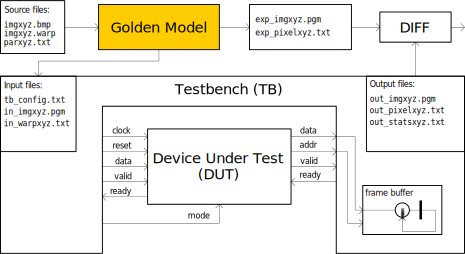
\includegraphics[width=\textwidth]{functional_verification_tb}
        \caption{Testbench used for functional verification.}%
        \label{fig:functional_verification_tb}
      \end{figure}

      Reference a ReadMe file that describes how the testbench can be launched.

    \subsubsection{Back-end implementation}

      In \gls{asic} projects, remember to discuss both front- and back-end implementation.
      That is, if you took special measures for floorplanning, \gls{dft}, or clock or power distribution, you will want to mention it here.
      In this case, make sure to add results that show the impact of your measures.

  \subsection{Results}

    Typical application-specific figures of merit of your hardware design are \gls{snr}, throughput, and memory/interface bandwidth.
    Moreover, you should also specify technology-specific figures such as area (for \glspl{asic}) or resource (for \glspl{fpga}) requirements, timing constraints, and power and energy consumption.

  \subsection{Data sheet}

    If your \gls{asic} is getting fabricated, you need to write a data sheet for it.
    You should put this data sheet into the appendix of your report.
    You are free to write the data sheet in a standalone document and include a \gls{pdf} file here or to write it in the source files of your report.

    Sections of a typical \gls{ic} data sheet are:
    \begin{itemize}
      \item Features
      \item Applications
      \item Packaging
      \item Bonding diagram like the one in \cref{fig:bonding_diagram}.
      \item Pinout diagram like the one in \cref{fig:asic_pinout}.
      \item Interface description
      \item Register map
      \item Operation modes:
      \begin{itemize}
        \item Functional modes
        \item Test modes
      \end{itemize}
      \item Electrical specifications
      \begin{itemize}
        \item Recommended operating regions
        \item Absolute maximum ratings
      \end{itemize}
    \end{itemize}

    \begin{figure}
      \centering
      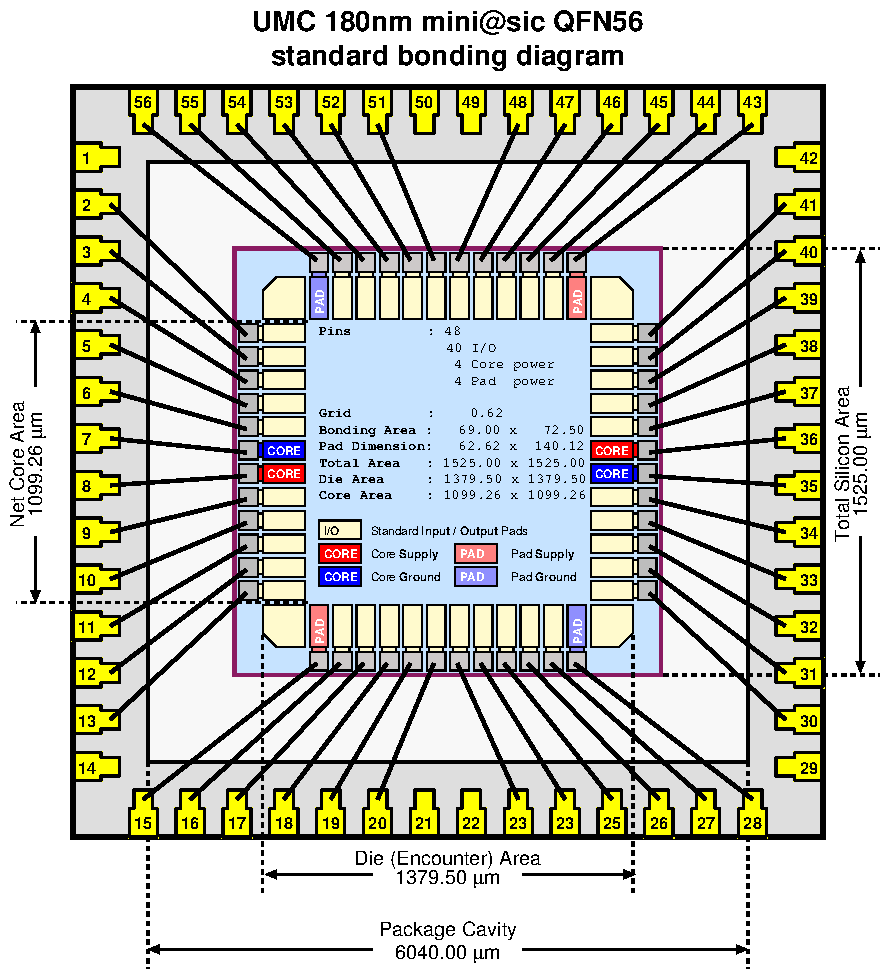
\includegraphics[width=.75\textwidth]{qfn56_180_std}
      \caption{Standard bonding diagram for QFN56 UMC 180\,nm mini@sics.}%
      \label{fig:bonding_diagram}
    \end{figure}

    \begin{figure}
      \centering
      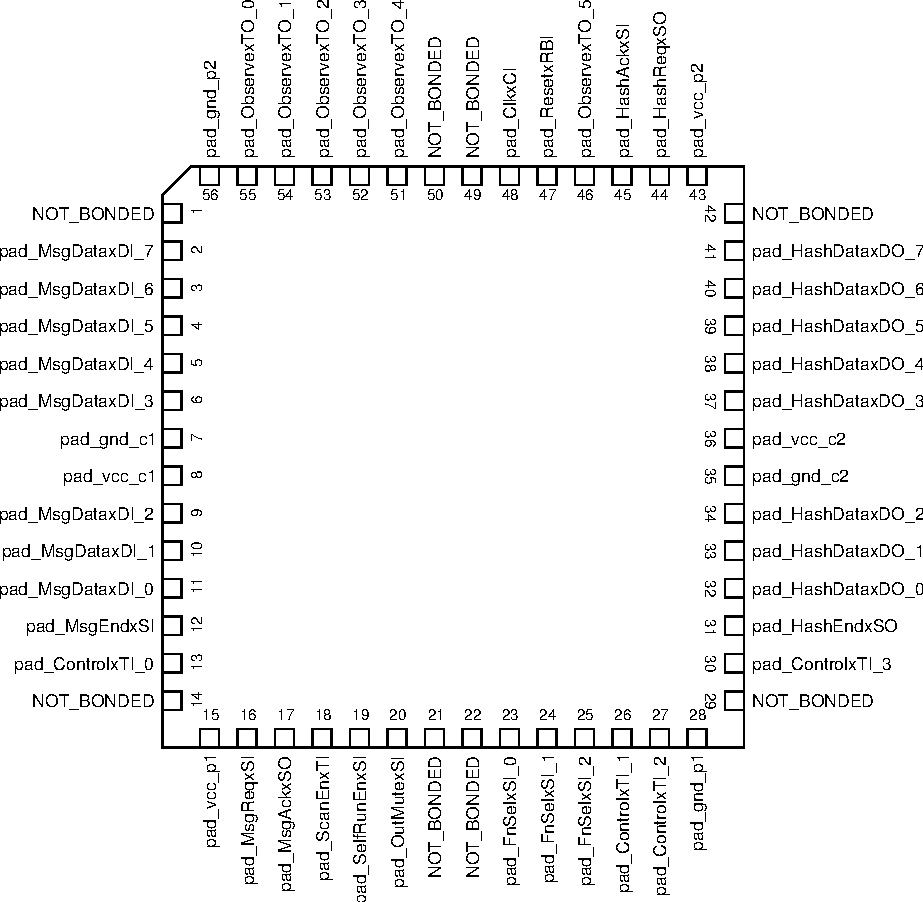
\includegraphics[width=.75\textwidth]{asic_pinout}
      \caption{Pinout for \textsc{MyFancyChip}.}%
      \label{fig:asic_pinout}
    \end{figure}

    For more information, up-to-date bonding diagrams, and other technology-specific data ask the \gls{dz}.
  % TODO: Remove these two appendices when you no longer need
% \chapter{Compact Guide to \LaTeX{} and the \textit{iisreport} Class}
\label{app:LaTeX_guide}

Writing a report with \LaTeX{} might at first not be as intuitive as with \gls{wysiwyg} editors.
However, once you get used to the (rather simple) syntax, you will soon discover how powerful it is and how it helps you achieve tasks that are very difficult (if not impossible) to achieve with \gls{wysiwyg} editors.

This report template provides everything you need to get you started working with \LaTeX{}.
The rest of this chapter contains a short guide with examples for commonly used features.

\section{Building the document}

  Generate a \gls{pdf} file from this template by simply executing \texttt{make} in the directory where the top-level \texttt{.tex} file is in.
  Internally, this will invoke the \texttt{latexmk} program, which is the simplest and most consistent way to build a \LaTeX{} document and is included in all recent \LaTeX{} distributions.
  Additionally, \texttt{make} will check the \texttt{fig/} directory and generate \gls{pdf} files for those figure raw files it knows how to compile (more on this in~\cref{sec:LaTeX_figures}).

\section{Text editing and spacing}

  White spaces and line breaks are automatically inserted when the document is compiled.
  For this, the number of spaces  between  two  words is irrelevant, but a different space length is automatically inserted after a period to make sentences better distinguishable.
  If you write a period that does not end a sentence, e.g., when mentioning Prof.\ Dr.\ S.\ Body, you need to escape the spaces between the abbreviated words with a backslash \verb|\|.
  If you want to prevent \LaTeX{} from breaking a line at a specific white space, you have to replace that space with a tilde \verb|~|.
  \LaTeX{} also automatically hyphenates English words, so it can break a line within a word, although it does so only cautiously.
  Automatic hyphenation can fail, e.g., for non-standard words, causing overly long lines.
  In such cases you have two options:
  First, if you have to break a standard word at an uncommon position, you can insert a \verb|\-| at that position in the word.
  Second, you can define the hyphenation of a non-standard word by adding \verb|\hyphenation{Jab-ber-woc-ky}| to the preamble\footnote{%
    The \emph{preamble} of a document is formed by all code between the \texttt{\textbackslash{}documentclass} command and the beginning of the document body after \texttt{\textbackslash{}begin\{document\}}.
  } of your document.

  A line of text is not broken at the same position as in the source code.
  For this reason, we suggest you put one sentence on one line of source code because this allows your \gls{vcs} to track content changes much better than if you wrap lines within sentences.
  To start a new paragraph, insert an empty line.
  You can manually break a line by writing \verb|\\|; however, this is rarely necessary and wide usage of it is a sign of fighting the typesetting system.

  By default in this template, paragraphs start with a short indentation and are not separated by vertical white space, but this can be changed.
  If you prefer the latter, pass the \texttt{parskip} option to the \texttt{iisreport} document class, i.e., change the first line of your main document to \verb|\documentclass[parskip]{iisreport}|.

  \subsection{Special characters}

    Many special characters are available, and they are all listed in \textsl{The Comprehensive \LaTeX{} Symbol List}~\cite{LaTeXSymbols}.
    At the beginning you might not know what to search for, though, so it can be more helpful to use the \textsl{Detexify}\footnote{\url{http://detexify.kirelabs.org/classify.html}} web app where you can draw the symbol you are looking for.

    A frequent mistake is to mix up the three dashes (-, --, and ---).
    The rules are simple~\cite{Knuth84}:
    \begin{itemize}
      \item The \emph{hyphen}, \verb|-|, is used between the elements of compound words; e.g., ``run-time''.
      \item The \emph{en-dash}, \verb|--|, is used for ranges; e.g., ``3--7''.
      \item The \emph{em-dash}, \verb|---|, is used for digressions within or at the end of a sentence---although you should use it sparingly.
    \end{itemize}

    Another frequent mistake are wrong quotation marks.
    Fortunately, this can also easily be avoided:
    Use \verb|`text'| for `single quotation marks' and \verb|``text''| for ``double quotation marks'' (have a look at the source code to see the matching pairs).
    In American English, double quotes prevail and single quotes are typically only used inside double quotes.

  \subsection{Font faces and emphasis}

    The font face can be changed locally with the commands in \cref{tbl:font_face_commands}.
    The text to appear differently has to be put between the curly braces \verb|{}|, i.e., the text is an \emph{argument} to one of the commands.
    Some font faces can also be combined by nesting them.
    For example, \verb|\textbf{\textit{some words}}| becomes \textbf{\textit{some words}}.

    \begin{table}
      \centerfloat
      \begin{tabular}{ l l }
        \toprule
        \textbf{Command} & \textbf{Output} \\
        \midrule
        \verb|\textrm{}| & \textrm{Roman (the default in this document)} \\
        \verb|\textsf{}| & \textsf{Sans serif} \\
        \verb|\texttt{}| & \texttt{Typewriter (i.e., all characters have the same width)} \\
        \verb|\textbf{}| & \textbf{Bold} \\
        \verb|\textit{}| & \textit{Italic} \\
        \verb|\textsl{}| & \textsl{Slanted} \\
        \verb|\textsc{}| & \textsc{Small caps} \\
        \bottomrule
      \end{tabular}
      \caption{Different font faces.}%
      \label{tbl:font_face_commands}
    \end{table}

    When you want to \emph{emphasize} text, use the \verb|\emph{}| command instead of one of the commands in \cref{tbl:font_face_commands}.
    In this way, you separate a \emph{property} of a piece of text (i.e., which text is emphasized) from its \emph{formatting} (i.e., how emphasized text looks like).
    This is an important principle in typesetting with \LaTeX{}.
    In this case, it allows you to define the formatting of all emphasized text independently of which text is meant to be emphasized.

  \subsection{Font sizes}

    The font size can be changed with the commands in \cref{tbl:font_sizes}.
    These commands change the size within a given \emph{scope}; for instance \verb|{\Large some words}| only prints ``some words'' large.

    \begin{table}
      \newcommand{\sampletext}{quick brown foxes}
      \centerfloat
      \begin{tabular}{ l l }
        \toprule
        \textbf{Command} & \textbf{Output sample} \\
        \midrule
        \verb|\tiny|          & {\tiny \sampletext} \\
        \verb|\scriptsize|    & {\scriptsize \sampletext} \\
        \verb|\footnotesize|  & {\footnotesize \sampletext} \\
        \verb|\small|         & {\small \sampletext} \\
        \verb|\normalsize|    & {\normalsize \sampletext} \\
        \verb|\large|         & {\large \sampletext} \\
        \verb|\Large|         & {\Large \sampletext} \\
        \verb|\LARGE|         & {\LARGE \sampletext} \\
        \verb|\huge|          & {\huge \sampletext} \\
        \verb|\Huge|          & {\Huge \sampletext} \\
        \bottomrule
      \end{tabular}
      \caption{Different font sizes.}%
      \label{tbl:font_sizes}
    \end{table}

  \subsection{Coloring text}

    \begin{figure}
      \centerfloat
      \begin{minipage}{1.1\textwidth}
        % Source: colors from `xcolor`, sorting by own implementation.
        \def\0#1{\colorbox{#1}{\phantom{XX}}~#1\\}
        \scriptsize
        \begin{multicols}{5}
          \noindent
          \0{Magenta}
          \0{Rhodamine}
          \0{VioletRed}
          \0{CarnationPink}
          \0{Lavender}
          \0{RubineRed}
          \0{WildStrawberry}
          \0{OrangeRed}
          \0{Salmon}
          \0{Maroon}
          \0{Red}
          \0{Mahogany}
          \0{BrickRed}
          \0{Melon}
          \0{RedOrange}
          \0{Sepia}
          \0{Brown}
          \0{Bittersweet}
          \0{RawSienna}
          \0{Peach}
          \0{Orange}
          \0{Tan}
          \0{Apricot}
          \0{BurntOrange}
          \0{YellowOrange}
          \0{Dandelion}
          \0{Goldenrod}
          \0{Yellow}
          \0{GreenYellow}
          \0{SpringGreen}
          \0{LimeGreen}
          \0{YellowGreen}
          \0{OliveGreen}
          \0{Green}
          \0{ForestGreen}
          \0{SeaGreen}
          \0{PineGreen}
          \0{JungleGreen}
          \0{Emerald}
          \0{TealBlue}
          \0{BlueGreen}
          \0{Aquamarine}
          \0{Turquoise}
          \0{SkyBlue}
          \0{Cyan}
          \0{ProcessBlue}
          \0{Cerulean}
          \0{MidnightBlue}
          \0{CornflowerBlue}
          \0{RoyalBlue}
          \0{NavyBlue}
          \0{CadetBlue}
          \0{Periwinkle}
          \0{Blue}
          \0{BlueViolet}
          \0{Violet}
          \0{RoyalPurple}
          \0{Purple}
          \0{Fuchsia}
          \0{Plum}
          \0{Orchid}
          \0{Mulberry}
          \0{DarkOrchid}
          \0{Thistle}
          \0{RedViolet}
        \end{multicols}
        \begin{multicols}{5}
          \noindent
          \columnbreak
          \0{black}
          \0{darkgray}
          \0{gray}
          \0{lightgray}
          \0{white}
        \end{multicols}
      \end{minipage}
      \caption{Selected predefined colors, sorted by hue.}%
      \label{fig:selected_colors}
    \end{figure}

    The color of text can be changed with the \verb|\textcolor| and \verb|\color| commands:
    The former takes two arguments, a declared color and the text to color.
    For example, \verb|\textcolor{RoyalBlue}{I am royal}| becomes \textcolor{RoyalBlue}{I am royal}.
    The latter takes only a defined color and colors all text in its scope.
    For example, \verb|{\color{RoyalPurple}So am I}| becomes {\color{RoyalPurple}So am I}.

    \Cref{fig:selected_colors} shows a selection of predefined colors.
    The \texttt{xcolor} package manual~\cite{xcolor} lists more colors and describes how to define custom colors.

\section{Debugging}

  Occasionally, you will make syntax mistakes while writing a document, causing compilation to fail.
  In this case, the last lines of the console output will mention an error and point you to a \texttt{.log} file in the directory where you ran \texttt{make}.
  Open that log file.
  Even though that file can be very long and contains many technical details that are of no interest to you, finding errors is easy: simply search for lines starting with an exclamation mark!

  If you use an undefined command, e.g., due to a typo, the error messages should be very helpful.
  If, however, you cause parentheses or environment delimiters to mismatch, the position of your mistake is hard to derive from the error messages.

  A good technique to locate a mistake is to comment out recent changes until the document compiles neatly again.
  For recompilation, you should use \texttt{make clean all} to prevent errors that crept into temporary files from disturbing your bug hunt.
  To reduce compilation time for large documents, you can comment out chapters that are known to be good.
  When you have a working version again, re-enable the code you commented out last piece-by-piece.
  This piecewise reduction should help you systematically find the mistake.

\section{Math mode}

  \LaTeX{} is probably the most powerful and elaborate tool to typeset mathematical content.
  Once you know a few core concepts, writing properly formatted mathematical content becomes quite simple.

  To distinguish maths from regular text, maths is written in \emph{math mode}.
  There are two categories that differ in their presentation: inline and displayed.
  Inline maths, e.g., $ a\sp{2} + b\sp{2} = c\sp{2} $ is enclosed in \verb|$| signs.
  It is meant for simple expressions.
  More complex content is displayed separately from the text.
  The most common way to display maths is inside the \texttt{equation} environment\footnote{%
    \emph{Environments} in \LaTeX{} are similar to commands, but are usually used for larger chunks of code.
    For example, the entire document except the preamble is inside the \texttt{document} environment.
    Environments are formed with \texttt{\textbackslash{}begin\{environmentname\}} \texttt{...} \texttt{\textbackslash{}end\{environmentname\}}.
  }, for example:
  \begin{equation}
    \int\sb{-\infty}\sp{\infty} x \dif x = 0.
  \end{equation}

  Subscripts are written with \verb|\sb{}|\footnote{%
    By default, \LaTeX{} would allow to use the underscore \texttt{_} for subscripts.
    In the \texttt{iisreport} document class, however, the underscore is a regular, printable character.
    The rationale is that the underscore is very common in technical designators and having to escape every single one is a common source of errors.
  }, superscripts with \verb|\sp{}|, integrals with \verb|\int|, and sums with \verb|\sum|.
  Have a look at the source code of the last paragraph for usage examples.

  Equations get a number by default, so you can label and refer to them (more on this in \cref{sec:cite_and_reference}).
  If you want to suppress an equation number, you can use the \emph{starred} version of the equation environment, i.e., \verb|equation*|.

  Many mathematical symbols and functions are predefined, letting you express relations such as $ \forall x \in \mathbb{R} $ $ \exists n \in \mathbb{N}: \ldots $ fluently.
  Wikipedia\footnote{\url{https://en.wikibooks.org/wiki/LaTeX/Mathematics\#List_of_Mathematical_Symbols}} has a list of all predefined mathematical symbols.

  Variable names are by default one character long, causing \verb|$ xy z $| to be typeset with identical spacing as \verb|$ xyz $|.
  You should thus use single-letter variables whenever possible.
  If you have to use multi-letter variables, write them inside the \verb|\var{}| command\footnote{%
    The \texttt{var} command is not standard \LaTeX{} but defined by the \texttt{iisreport} document class.
    If you want to use it elsewhere, it is very simple to implement: \url{https://tex.stackexchange.com/a/129434/92384}.
  }.
  This causes $ x $ and $ y $ in the two-letter variable $ \var{xy} $ to be closer together.
  To make the variable clearly distinguishable from the next one, however, you may still have to insert a space\footnote{%
    The most common horizontal spacing macros in math mode are (in increasing order):
    \texttt{\textbackslash{},}, \texttt{\textbackslash{};}, \texttt{\textbackslash{}enspace}, \texttt{\textbackslash{}quad}, and \texttt{\textbackslash{}qquad}.
    A complete list with examples is available here: \url{https://tex.stackexchange.com/a/74354/92384}.
    Keep in mind that frequent insertion of manual spacing may be a hack around a more fundamental problem.
  } (as in $ \var{xy} \, z $) or even an operator (as in $ \var{xy} \cdot z $).

  When you want to use text in math mode (subscripts are a common use case for this), you must write that text inside the \verb|\text{}| command to avoid the same problems as with multi-letter variables.

  \subsection{Delimiters: Parentheses, brackets, bars, and intervals}

    For simple parentheses and square brackets, you can readily use the \texttt{()} and \texttt{[]} characters, respectively.
    Curly braces are a bit more involved because \verb|{}| are grouping characters.
    Thus, you would have to escape them and write \verb|\{\}| instead.
    However, we recommend to use the \verb|\cbr{}| command (short for ``curly braces'') instead.
    That command has the additional advantage of automatically sizing parentheses to the content.
    (The automatic sizing can be disabled by passing \verb|[0]| as optional first argument to the command.)
    If you need automatically sized parentheses and square brackets, the commands are \verb|\del{}| (for ``delimiter'') and \verb|\sbr{}| (for ``square bracket''), respectively.
    This allows you to effortlessly maintain readability even in deeply nested equations:
    \begin{equation}
      \del{E\sbr{\min\cbr{X\sb{1}, X\sb{2}}} - \del{\pi - \arccos\del{\frac{y}{r}}}}\sp{n}.
    \end{equation}

    Absolute values are written with \verb|\abs{}|, e.g.,
    \begin{equation}
      \abs{\exp\del{x \pi i}} = 1 \quad\forall x \in \mathbb{R},
    \end{equation}
    while vector norms are written with \verb|\norm{}|, e.g.,
    \begin{equation}
      \norm{\vec{x}}\sb{2} = \sqrt{\sum\sb{k=1}\sp{n} x\sb{k}\sp{2}} \quad\forall \vec{x} \in \mathbb{R}\sp{n},
    \end{equation}
    where the vector $ \vec{x} $ was written with \verb|\vec{x}| and the square root with \verb|sqrt{..}|.

    Intervals are written with the \verb|\intxy{}| commands, where each of \texttt{x} and \texttt{y} are either \texttt{o} for open or \texttt{c} for closed.

  \subsection{Differential and derivative operators}

    Differential and derivative operators are written with the following commands:
    \verb|\dif x| is the simple differential operator, e.g., $ \dif x $.
    \verb|\Dif x| is a derivative operator, e.g., $ \Dif x $.
    \verb|\od[n]{f}{x}| is the ordinary $n$-th derivative operator, e.g., $ \od[n]{f}{x} $.
    \texttt{n} is optional and should be omitted for the first derivative.
    \verb|\pd[n]{f}{x}| is the partial $n$-th derivative operator, e.g., $ \pd[n]{f}{x} $.
    Finally, \verb|\md{f}{n}{x}{q}{y}{r}| is the mixed partial derivative operator, e.g., $ \md{f}{n}{x}{q}{y}{r} $, where \texttt{n} is the total order of differentiation and \texttt{q} and \texttt{r} are the orders of differentiation for \texttt{x} and \texttt{y}, respectively.

  \subsection{Vectors, matrices, and distinction of cases}

    Both vectors and matrices are written with the \texttt{Xmatrix} environments, where \texttt{X} defines the delimiter of the matrix and can be \texttt{p} for parentheses, \texttt{b} for brackets, \texttt{B} for curly braces, \texttt{v} for vertical bars, \texttt{V} for double vertical bars, or omitted for no delimiters.
    The matrix is written row-wise with the elements of a row separated by \verb|&| and each row is terminated by \verb|\\|.
    A column vector is just a matrix with one column, a row vector one with one row.
    For example:
    \begin{equation}
      x = \begin{pmatrix}
        x\sb{1} & x\sb{2} \\
      \end{pmatrix}
      \quad
      y = \begin{pmatrix}
        y\sb{1} \\
        y\sb{2} \\
      \end{pmatrix}
      \quad
      A = \begin{pmatrix}
        a\sb{1,1} & a\sb{1,2} \\
        a\sb{2,1} & a\sb{2,2} \\
      \end{pmatrix}
    \end{equation}

    The \texttt{Xmatrix} environments center the columns by default.
    If you want a different alignment, use the starred variant\footnote{%
      The \emph{starred variant} of an environment or a command simply has a star \texttt{*} at the end of the environment or command name, respectively.
      Not all environments and commands have a starred variant.
    } of the environments, which accepts a single character as optional argument\footnote{%
      \emph{Optional arguments} are always enclosed in square brackets \texttt{[]}.
    }: \texttt{r} for right, \texttt{c} for center, and \texttt{l} for left.

    To write case distinctions, use the \texttt{dcases} environment.
    For example:
    \begin{equation}
      a(v) =
      \begin{dcases}
        0             & \text{if } v \geq \mathrm{c}, \\
        \epsilon > 0  & \text{else}.
      \end{dcases}
    \end{equation}
    If you want the curly brace to be on the right of the cases, use the \texttt{rcases} environment.

  \subsection{Multi-line equations}

    If you want to write a single equation that is longer than one line, use the \texttt{multline} (without `i'!) environment.
    That environment switches to math mode by itself, so you \emph{must not} use it inside \texttt{equation}.
    Use the line break command, \verb|\\|, to define the two lines of the equation.
    For example:
    \begin{multline}
      \alpha + \beta + \gamma + \delta + \epsilon + \zeta + \eta + \theta + \iota + \kappa + \lambda + \mu + \nu + \xi + + \pi + \rho + \sigma + \tau \\
       = \upsilon + \phi + \chi + \psi + \omega.
    \end{multline}

    To write multiple equations in series or an especially complicated multi-line equation, use the \texttt{IEEEeqnarray} environment.
    That environment takes a series of characters specifying the columns as argument.
    The most common argument is \texttt{rCl}, meaning one right-aligned column followed by a center-aligned separator followed by a left-aligned column.
    As with matrices, use \verb|&| to separate columns and \verb|\\| to separate equation lines.
    For example:
    \begin{IEEEeqnarray}{rCl}
      a & = & b + c \\
        & = & d + e + f + g + h + i + j + k \nonumber\\
        &   & +\> l + m + n + o \\
        & = & p + q + r + s,
    \end{IEEEeqnarray}
    where the first line of the second equation was ended by \verb|\nonumber| to suppress numbering that part of the equation.

    Browse through \textsl{How to Typeset Equations in \LaTeX{}}~\cite{LaTeXEquations} for further informations and solutions to more complex examples.

  \subsection{Definitions, theorems, lemmas, and proofs}

    Here are some examples on writing definitions, theorems, lemmas, and proofs.

    \begin{definition}[Singularity]
      Let $ U $ be an open subset of the complex numbers $ \mathbb{C} $, $ a \in U $, and $ f $ be a complex differentiable function defined on $ U \setminus \cbr{a} $.

      The point $ a $ is a \emph{removable singularity} of $ f $ if there exists a holomorphic function $ g $ defined on all of $ U $ such that $ f(z) = g(z) \>\forall z \in U \setminus \cbr{a} $.

      The point $ a $ is a \emph{pole} or \emph{non-essential singularity} of $ f $ if there exists a holomorphic function $ g $ defined on $ U $ with $ g(a) \neq 0 $ and $ n \in \mathbb{N} $ such that
      \begin{equation}
         f(z) = \frac{g(z)}{(z - a)\sp{n}} \quad\forall z \in U \setminus \cbr{a}.
      \end{equation}
      The lowest such number $ n $ is called the \emph{order of the pole}.

      The point $ a $ is an \emph{essential singularity} of $ f $ if it is neither a removable singularity nor a pole.
      The point $ a $ is an essential singularity iff the Laurent series has infinitely many powers of negative degree.
    \end{definition}

    \begin{theorem}[Residue Theorem]
      Let $ f $ be analytic in the region $ G $ except for the isolated singularities $ a\sb{1} $, $ a\sb{2} $, \ldots, $ a\sb{m} $.
      If $ \gamma $ is a closed rectifiable curve in $ G $ that does not pass through any of the points $ a\sb{k} $ and if $ \gamma \approx 0 $ in $ G $, then
      \begin{equation}
        \frac{1}{2 \pi i} \int\sb{\gamma} f = \sum\sb{k = 1}\sp{m} n(\gamma; a\sb{k}) \,\text{Res}(f; a\sb{k}).
      \end{equation}
    \end{theorem}

    \begin{proof}
      Left as an exercise for the reader.
    \end{proof}

    \begin{lemma}[Schwarz]
      Let $ D \coloneqq \cbr{z \in \mathbb{C}: \abs{z} < 1} $ be the open unit disk in the complex plane centered at the origin, and let $ f: D \to \mathbb{C} $ be a holomorphic map such that $ f(0) = 0 $ and $ \abs{f(z)} \leq 1 $ on $ D $.
      Then, $ \abs{f(z)} \leq \abs{z} \>\forall z \in D $ and $ \abs{f'(0)} \leq 1 $.
      Moreover, if $ \abs{f(z)} = \abs{z} $ for some $ z \neq 0 $ or $ \abs{f'(0)} = 1 $, then $ f(z) = a z $ for some $ a \in \mathbb{C} $ with $ \abs{a} = 1 $.
    \end{lemma}

    \begin{proof}
      Beyond the scope of this document.
    \end{proof}

\section{Quantities with SI units}

  \begin{itemize}
    \item quantity with a unit: \SI{300}{\mega\hertz}
    \item unit alone: \si{\giga\volt}
    \item ranges of quantities with units: \SIrange{2}{256}{\mebi\bit\per\second}
    \item number (especially for engineering notation or very large numbers): \num{10000}, \num{3.14e6}, \num{5e-12}
    \item ranges of numbers \numrange{5e-12}{3.14e6}
  \end{itemize}

  Math mode not required, but can be used with it.

\section{Enumerations and itemizations}

  Itemizations are \ldots
  \begin{itemize}
    \item unnumbered and
    \item written inside the \texttt{itemize} environment, where every item starts with \verb|\item|.
  \end{itemize}

  Enumerations, on the other hand, are \ldots
  \begin{enumerate}
    \item numbered and
    \item written inside the \texttt{enumerate} environment.
  \end{enumerate}

  Both itemizations and enumerations can be nested.
  The indentation level and itemization items are then automatically adjusted:
  \begin{enumerate}
    \item This demonstrates that
    \begin{enumerate}
      \item enumerations and
      \item itemizations
      \begin{itemize}
        \item can be nested.
      \end{itemize}
    \end{enumerate}
  \end{enumerate}

\section{Floats: figures and tables}
\label{sec:LaTeX_figures}

  Both figures and tables normally form \emph{floating} environments.
  This means that \LaTeX{} will automatically place them near to where they were in the source code, but not at the exact same position.
  The placement algorithm is fairly sophisticated~\cite{LaTeXFloatPlacement} and usually works reasonably well.

  The base environment for figures is \texttt{figure}, the one for tables is \texttt{table}.
  Floats usually get a caption with the \verb|\caption{}| command.
  If you want to refer to them (more on this in \cref{sec:cite_and_reference}), you additionally have to put a \verb|\label{}| after the \verb|\caption{}| but on the same line (to have correct page numbers even near page breaks).

  To center-align the content of a float, use the \verb|\centerfloat| command at the beginning of that float.

  \subsection{Figures}

    Images can be included with the \verb|\includegraphics[properties]{file_name}| command, where \texttt{properties} allows to, e.g., define the \texttt{width}, \texttt{height}, or \texttt{scale} of an image in the \texttt{key=value} syntax.
    The \texttt{file_name} is relative to the \texttt{fig/} directory and the default suffix, \texttt{.pdf}, can be omitted.
    An example figure is given in \cref{fig:example_figure}.

    \begin{figure}
      \centerfloat
      
\includegraphics[width=5cm]{eth_logo}
      % Note: We do not have the SVG source file for the image above, so we have to put the PDF under version control.
      \caption{Example figure.}%
      \label{fig:example_figure}
      % Note: The `\label{}` can be on the line after the `\caption{}` if the `\caption{}` line ends with a comment.
    \end{figure}

    Whenever possible, you should use \glspl{svg} for two reasons:
    First, they can be scaled losslessly to the target size and resolution.
    Second, they allow you to keep a small, modifiable source file of the graphic under version control and have the \gls{pdf} file to be included built automatically.

    We recommend using \textsl{Inkscape}\footnote{Freely available at \url{https://inkscape.org}.}.
    Simply draw a figure in Inkscape, set the canvas to where you want the image border, save the original \texttt{.svg} file in the \texttt{fig/} directory, and use \verb|\includegraphics| on the file name without suffix.
    When you run \texttt{make}, the corresponding \gls{pdf} file will get built automatically and included in your document.
    If you use a \gls{vcs} (we highly recommend to do so!), track the original \texttt{.svg} file but add the auto-built \texttt{.pdf} file to the ignore list (e.g., \texttt{fig/.gitignore}).
    If you include \gls{pdf} files of which you have no source files, track that \texttt{.pdf} file in your \gls{vcs}.

    As Inkscape does not support embedding fonts in its \gls{svg} files, you should either only use standard, widely-available fonts\footnote{\href{https://www.w3schools.com/cssref/css_websafe_fonts.asp}{Web safe fonts} are good candidates for widely available fonts.} or track the auto-built \gls{pdf} images in \texttt{fig/} with your \gls{vcs}.
    If you choose the latter, though, be aware that other collaborators who do not have the font installed must not commit changes to the built \gls{pdf} images (because text with missing fonts will be rendered incorrectly by their Inkscape).

  \subsection{Tables}

    \begin{table}
      \centerfloat
      \begin{tabular}{ r r r r }
        \toprule
        \textbf{Decimal} & \textbf{Hexadecimal} & \textbf{Octal} & \textbf{Binary} \\
        \midrule
        10 & $ \mathtt{A}\sb{16} $ & $ \mathtt{12}\sb{8} $ & $ \mathtt{1010}\sb{2} $ \\
        13 & $ \mathtt{D}\sb{16} $ & $ \mathtt{15}\sb{8} $ & $ \mathtt{1101}\sb{2} $ \\
        \bottomrule
      \end{tabular}
      \caption{Simple example table with some values in different number systems.}%
      \label{tbl:sample_number_systems}
    \end{table}

    \begin{table}
      \centerfloat
      \rowcolors{2}{lightgray}{white}
      \begin{tabular}{ c c c }
        \toprule
        \textbf{Some} & \textbf{title} & \textbf{words} \\
        \midrule
        odd   & odd & odd \\
        even  & \cellcolor{darkgray}\color{white} even  & even  \\
        odd   & odd & odd \\
        \bottomrule
      \end{tabular}
      \caption{Simple example table with different row and cell colors.}%
      \label{tbl:sample_colors}
    \end{table}

    \begin{table}
      \centerfloat
      \begin{tabular}{ l p{1.5cm} p{1.5cm} p{7cm} }
        \toprule
        \textbf{Day} & \textbf{Min.\ Temp.} & \textbf{Max.\ Temp.} & \textbf{Description} \\
        \midrule
        Monday  & \SI{11}{\degreeCelsius} & \SI{22}{\degreeCelsius} & A clear day with lots of sunshine. However, a strong breeze will bring down the temperatures. \\
        Tuesday & \SI{9}{\degreeCelsius}  & \SI{19}{\degreeCelsius} & Cloudy with rain across many northern regions.  Clear spells across most of Scotland and Northern Ireland, but rain reaching the far northwest. \\
        \bottomrule
      \end{tabular}
      \caption{%
        Example table with fixed column widths: \SI{1.5}{\centi\meter} for columns two and three, \SI{7}{\centi\meter} for column four.
        Content adopted from \href{https://en.wikibooks.org/wiki/LaTeX/Tables\#Text_wrapping_in_tables}{Wikibooks}.
      }%
      \label{tbl:fixed_width_columns}
    \end{table}

\section{Algorithms and source code listings}

  \Cref{alg:disjoint_decomposition} shows an example algorithm.
  Have a look at the source code to discover how it works.

  \begin{algorithm}
    \SetKwData{Left}{left}\SetKwData{This}{this}\SetKwData{Up}{up}
    \SetKwFunction{Union}{Union}\SetKwFunction{FindCompress}{FindCompress}
    \SetKwInOut{Input}{input}\SetKwInOut{Output}{output}

    \Input{A bitmap $Im$ of size $w\times l$}
    \Output{A partition of the bitmap}
    \BlankLine
    \emph{special treatment of the first line}\;
    \For{$i\leftarrow 2$ \KwTo $l$}{
      \emph{special treatment of the first element of line $i$}\;
      \For{$j\leftarrow 2$ \KwTo $w$}{\label{forins}
        \Left$\leftarrow$ \FindCompress{$Im[i,j-1]$}\;
        \Up$\leftarrow$ \FindCompress{$Im[i-1,]$}\;
        \This$\leftarrow$ \FindCompress{$Im[i,j]$}\;
        \If(\tcp*[h]{O(\Left,\This)==1}){\Left compatible with \This}{\label{lt}
          \lIf{\Left $<$ \This}{\Union{\Left,\This}}
          \lElse{\Union{\This,\Left}}
        }
        \If(\tcp*[f]{O(\Up,\This)==1}){\Up compatible with \This}{\label{ut}
          \lIf{\Up $<$ \This}{\Union{\Up,\This}}
          \tcp{\This is put under \Up to keep tree as flat as possible}\label{cmt}
          \lElse{\Union{\This,\Up}}\tcp*[r]{\This linked to \Up}\label{lelse}
        }
      }
      \lForEach{element $e$ of the line $i$}{\FindCompress{p}}
    }
    \caption{Disjoint decomposition.}%
    \label{alg:disjoint_decomposition}
  \end{algorithm}

  Source code listings are written inside the \texttt{lstlisting} environment, which takes optional arguments such as the \texttt{language} of the code, a \texttt{caption}, and a \texttt{label} in \verb|key=value| syntax.
  \Cref{lst:simple_C} shows an example listing.

  \begin{lstlisting}[language=C, caption={Simple C code snippet.}, label={lst:simple_C}]
    int main()
    {
      return 0;
    }
  \end{lstlisting}

  External source code files can be included as listing with the \verb|\lstinputlisting{}| command.
  Since you rarely want to include an entire file, you can specify the first and the last line with the \texttt{firstline} and the \texttt{lastline} key, respectively.

\section{Citing and referencing}
\label{sec:cite_and_reference}

  Use the \verb|\cref{}| command to reference a document-internal label.
  Use the \verb|\cite{}| command to cite an entry in the bibliography.
  You should always use a nonbreaking space, \verb|~|, before the \verb|\cite{}| command to prevent the citation label from falling to the next line.

\section{Printing and binding}

  When printing this document, pass the \texttt{print} option to the \texttt{iisreport} class.
  This will cause the layout to be optimized for printing.

\section{Further reading}

  For a guide on writing research reports, we recommend the \textsl{Manual for Writers of Research Papers, Theses, and Dissertations}~\cite{Turabian13}.
  Furthermore, \textsl{The Elements of Style}~\cite{Strunk12} and \textsl{The Chicago Manual of Style}~\cite{ChicagoManualOfStyle} are useful guides on concise writing in general.
  The latter is freely available online within the ETH network.\footnote{\url{http://www.chicagomanualofstyle.org}}

  If you are interested to learn more about \LaTeX{}, you will find many resources online but the majority of them are written by casual amateurs and can teach you bad practices.
  Their approach is not strictly wrong but in the long term can cost you a lot of time compared to proper solutions.
  Thus, let us suggest to start all your \TeX{}-related searches at the \TeX{} StackExchange\footnote{\url{https://tex.stackexchange.com/}} community.
  Especially in the beginning, you will encounter common problems, for which there are usually several high-quality solutions on StackExchange, complete with an explanation of why the problem arose.

  There are also some very good books on \LaTeX{}.
  \textsl{The Not So Short Introduction to \LaTeX2e{}}~\cite{LaTeXIntroduction} is an excellent start, and \textsl{More Math into \LaTeX{}}~\cite{Graetzer16} teaches \SI{99}{\percent} of what you need to know about typesetting maths.
  The first book\footnote{\url{http://tobi.oetiker.ch/lshort/lshort.pdf}} and the first section of the second book\footnote{\url{http://www.ctan.org/tex-archive/info/Math_into_LaTeX-4/Short_Course.pdf}} are freely available online.
  For more advanced users, \textsl{The \LaTeX{} Companion}~\cite{Mittelbach04} and the \textsl{The \TeX{}book}~\cite{Knuth84} are the definitive books.

\section{\textit{iisreport} options quick reference}

  The \textit{iisreport} document class offers a few options that allow you to easily customize the layout of your report and configure certain features.
  Options can be specified inside the square brackets on the first line of the \texttt{report.tex} file, with individual options separated by commas.
  Here is an overview of all available options in alphabetic order:

  \begin{itemize}[itemsep=0pt]
    \item \texttt{oldfonts} brings back the fonts from the legacy \acrshort{iis} report template.
    \item \texttt{oldsubscript} disables making the underscore printable and makes it usable for subscripts instead.
    \item \texttt{parskip} causes paragraphs to start with a vertical space of half a line instead of indentation.
    \item \texttt{print} optimizes the page layout for printing and binding.
  \end{itemize}
          % their guidelines.
\chapter{Task Description}

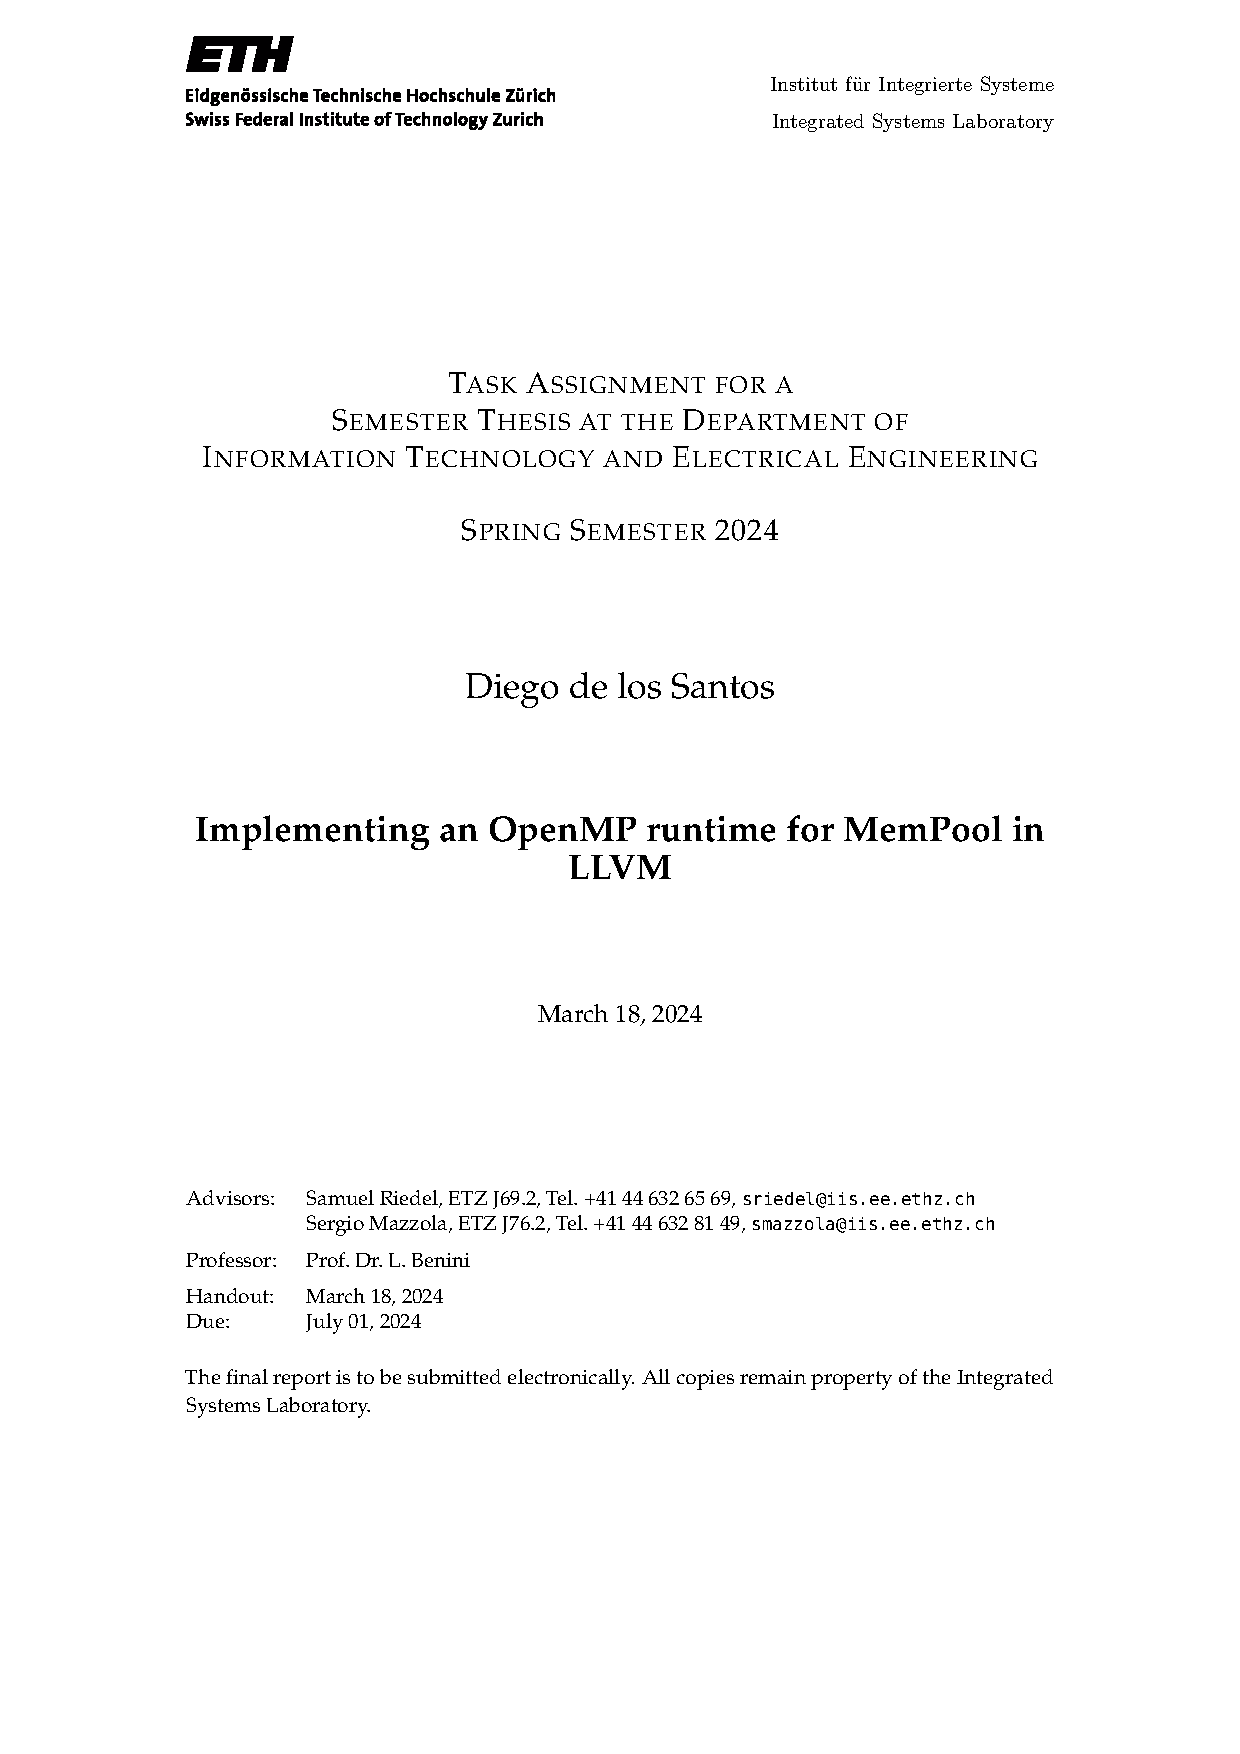
\includepdf[pages=-, scale=0.9]{./fig/MemPool_KMP_Task_Description.pdf}


\backmatter

\listofacronyms

\listoffigures
\listoftables

% TODO: Remove the `latex_and_writing` bibliography when you no longer need that guide.
\bibliography{./bib/main}

\end{document}
